%                                                                 aa.dem
% AA vers. 8.2, LaTeX class for Astronomy & Astrophysics
% demonstration file
%                                                       (c) EDP Sciences
%-----------------------------------------------------------------------
%
%\documentclass[referee]{aa} % for a referee version
%\documentclass[onecolumn]{aa} % for a paper on 1 column  
%\documentclass[longauth]{aa} % for the long lists of affiliations 
%\documentclass[rnote]{aa} % for the research notes
%\documentclass[letter]{aa} % for the letters 
%\documentclass[bibyear]{aa} % if the references are not structured 
% according to the author-year natbib style

%%%%%%%%%%%%%%%%%%%%%%%%%%%%%%%%%%%%%%%%%%%%%%%%%%%%%%%%%%%%%%%%%%%%%%%%%%%%
\documentclass{aa}    %% Astronomy & Astrophysics style class aa.cls v8.2
%\documentclass[referee]{aa} 

\usepackage{graphicx,url,twoopt,natbib}
\usepackage[varg]{txfonts}           %% A&A font choice

\usepackage{pdfcomment}              %% for popup acronym meanings
\usepackage{acronym}                 %% for popup acronym meanings

\usepackage{url}
\usepackage{color,hyperref}
\definecolor{linkcolor}{rgb}{0,0.3,0.7}
\hypersetup{colorlinks=true,
	linkcolor=linkcolor, 
	citecolor=linkcolor,
	filecolor=linkcolor, 
	urlcolor=linkcolor}

\usepackage{natbib}

\bibpunct{(}{)}{,}{a}{}{,}    %% natbib cite format used by A&A and ApJ

% Manually specified definitions
\newcommand{\farc}{\hbox{$.\!\!^{\prime\prime}$}} 
\newcommand{\ergA}{$\rm{erg\,cm^{-2}\,s^{-1}\,\AA^{-1}}$} 
\newcommand{\erg}{$\rm{erg\,cm^{-2}\,s^{-1}}$} 
\newcommand{\kms}{$\rm{km\,s^{-1}}\,$}

\newcommand{\griz}{$g' r' i' z'$}
\newcommand{\JHK}{$JHK_{\rm{s}}$}
\newcommand{\gK}{$g' r' i' z' JHK_{\rm{s}}$}
\newcommand{\Msun}{$M_\odot$}


% Elements
\newcommand{\lya}{Ly$\alpha$} 
\newcommand{\lyb}{Ly$\beta$} 
\newcommand{\lyg}{Ly$\gamma$} 
\newcommand{\hb}{H$\beta$} 
\newcommand{\ha}{H$\alpha$} 
\newcommand{\hg}{H$\gamma$} 
\newcommand{\hi}{\ion{H}{i}} 
\newcommand{\hei}{[\ion{He}{i}]} 
\newcommand{\oi}{[\ion{O}{i}]} 
\newcommand{\sii}{[\ion{S}{ii}]} 
\newcommand{\siii}{[\ion{S}{iii}]} 
\newcommand{\oii}{[\ion{O}{ii}]} 
\newcommand{\oiii}{[\ion{O}{iii}]}
\newcommand{\nii}{[\ion{N}{ii}]} 
\newcommand{\nv}{[\ion{N}{v}]} 
\newcommand{\neiii}{[\ion{Ne}{iii}]} 
\newcommand{\NIii}{[\ion{Ni}{ii}]} 
\newcommand{\feii}{\ion{Fe}{ii}} 
\newcommand{\civ}{\ion{C}{iv}} 
\newcommand{\cii}{\ion{C}{ii}}
\newcommand{\mgi}{\ion{Mg}{i}} 
\newcommand{\mgii}{\ion{Mg}{ii}} 
\newcommand{\ali}{\ion{Al}{i}} 
\newcommand{\alii}{\ion{Al}{ii}} 
\newcommand{\aliii}{\ion{Al}{iii}} 
\newcommand{\SIi}{\ion{Si}{i}} 
\newcommand{\SIii}{\ion{Si}{ii}} 
\newcommand{\SIiii}{\ion{Si}{iii}} 
\newcommand{\SIiv}{\ion{Si}{iv}} 
\newcommand{\znii}{\ion{Zn}{ii}} 
\newcommand{\crii}{\ion{Cr}{ii}} 
\newcommand{\mnii}{\ion{Mn}{ii}} 
\newcommand{\tiii}{\ion{Ti}{ii}} 
\newcommand{\caii}{\ion{Ca}{ii}} 


\usepackage{xcolor}
\newcommand\todo[1]{\textbf{(#1)}}

\begin{document}
	
\title{The host galaxy of the short GRB~111117A at $z = 2.211$: impact on the short GRB redshift distribution and progenitor channels\thanks{Based on observations collected at ESO/VLT under programme 088.A-0051 and 091.D-0904, at TNG under programme A24TAC\_38, at Gemini North under programme GN-2011B-Q-10 and GTC under programme GTC43-11B.}}

\titlerunning{GRB~111117A}


\author{J.~Selsing\inst{1}
\and T.~Kr\"{u}hler\inst{2}
\and D.~Malesani\inst{1}
\and P.~D'Avanzo\inst{3}
\and S.~Schulze \inst{4, 5, 6}
\and S.~D.~Vergani\inst{3, 7}
\and J.~Palmerio\inst{8}
\and J.~Japelj\inst{9}
\and B.~Milvang-Jensen\inst{1}
\and D.~Watson\inst{1}
\and P.~Jakobsson\inst{10}
%
\and J.~Bolmer \inst{2}
\and Z.~Cano\inst{11}
\and S.~Covino \inst{3}
%\and L.~B.~Christensen\inst{1}
\and V.~D'Elia\inst{12, 13}
\and A.~de~Ugarte~Postigo\inst{11, 1}
\and J.~P.~U.~Fynbo\inst{1}
\and A.~Gomboc\inst{14}
\and K.~E.~Heintz\inst{10,1}
\and L.~Kaper \inst{9}
\and A.~J.~Levan \inst{15}
\and S.~Piranomonte \inst{12}
\and G.~Pugliese \inst{9}
\and R.~S\'{a}nchez-Ram\'{\i}rez \inst{11, 17}
\and M.~Sparre\inst{1,18}
\and N.~R.~Tanvir\inst{19}
\and C.~C.~Th\"{o}ne\inst{11}
\and K.~Wiersema \inst{19}
}


\institute{Dark Cosmology Centre, Niels Bohr Institute, University of Copenhagen, Juliane Maries Vej 30, 2100 K\o benhavn \O, Denmark
%2
\and Max-Planck-Institut f\"{u}r extraterrestrische Physik, Giessenbachstra\ss e, 85748 Garching, Germany
%3
\and INAF - Osservatorio Astronomico di Brera, via E. Bianchi 46, I-23807, Merate (LC), Italy
%4
\and Instituto de Astrof\'isica, Facultad de F\'isica, Pontificia Universidad Cat\'olica de Chile, Vicu\~{n}a Mackenna 4860, 7820436 Macul, Santiago, Chile
%5
\and Millennium Institute of Astrophysics, Vicu\~{n}a Mackenna 4860, 7820436 Macul, Santiago, Chile
%6
\and Department of Particle Physics and Astrophysics, Faculty of Physics, Weizmann Institute of Science, Rehovot 76100, Israel
%7
\and GEPI, Observatoire de Paris, PSL Research University, CNRS, Place Jules Janssen, 92190 Meudon, France
%8
\and Sorbonne Universités, UPMC Univ. Paris 6 et CNRS, UMR 7095, Institut d’Astrophysique de Paris, 98 bis bd Arago, 75014 Paris, France
%9
\and Anton Pannekoek Institute for Astronomy, University of Amsterdam, Science Park 904, 1098 XH Amsterdam, The Netherlands
%10
\and Centre for Astrophysics and Cosmology, Science Institute, University of Iceland, Dunhagi 5, 107 Reykjav\'ik, Iceland
%11
\and Instituto de Astrof\'isica de Andaluc\'ia (IAA-CSIC), Glorieta de la Astronom\'ia s/n, E-18008, Granada, Spain
%12
\and INAF-Osservatorio Astronomico di Roma, Via Frascati 33, I-00040 Monteporzio Catone, Italy
%13
\and ASI-Science Data Centre, Via del Politecnico snc, I-00133 Rome, Italy
%14
\and Centre for Astrophysics and Cosmology, University of Nova Gorica, Vipavska 13, 5000 Nova Gorica, Slovenia.
%15
\and Department of Physics, University of Warwick, Coventry CV4 7AL, UK
%16
\and INAF, Osservatorio Astronomico di Brera, Via E. Bianchi 46, I-23807 Merate (LC), Italy
%17
\and Istituto de Astrofisica e Planetologia Spaziali, INAF, Via Fosso del Cavaliere 100, I-00133 Roma, Italy
%18
\and Heidelberger Institut f{\"u}r Theoretische Studien, Schloss-Wolfsbrunnenweg 35, 69118 Heidelberg, Germany 
%19
\and Department of Physics \& Astronomy and Leicester Institute of Space \& Earth Observation,
University of Leicester, University Road, Leicester, LE1 7RH, UK
}


\date{Received/ accepted}


\authorrunning{Selsing et al.}


\abstract{
It is notoriously difficult to localize short $\gamma$-ray bursts (sGRBs) and
their hosts to measure their redshifts. These measurements, however, are
critical to constrain the nature of sGRB progenitors, their redshift
distribution and the $r$-process element enrichment history of the universe.
Here, we present spectroscopy of the host galaxy of GRB~111117A and measure its
redshift to be $z = 2.211$. This makes GRB~111117A the most distant
high-confidence short duration GRB detected to date. Our spectroscopic redshift
supersedes a lower, previously estimated photometric redshift value for this
burst.

We use the spectroscopic redshift, as well as new imaging data to constrain the
nature of the host galaxy and the physical parameters of the GRB. The rest-frame
X-ray derived hydrogen column density, for example, is the highest compared to a
complete sample of sGRBs and seems to follow the evolution with redshift as
traced by the hosts of long GRBs.

The host lies in the brighter end of the expected sGRB host brightness
distribution at $z = 2.211$, and is actively forming stars. Using the observed
sGRB host luminosity distribution, we find that between 43 and 71 per cent of
all \textit{Swift}-detected sGRBs have too faint hosts at $z\sim2$ to allow for
a secure redshift determination. This implies that the measured sGRB redshift
distribution could be incomplete at high redshift. The large $z$ of
GRB~111117A is evidence against a lognormal delay-time model for sGRBs through
the predicted redshift distribution of sGRBs, which is very sensitive to
high-$z$ sGRBs.

From the age of the universe at the time of GRB explosion, an initial neutron
star (NS) separation of $a_0 < 3.1~R_\odot$ is required in the case where the
progenitor system is a circular pair of inspiralling NSs. This constraint
excludes some of the longest sGRB formation channels for this burst.
}

\keywords{gamma-ray burst: individual: GRB~111117A -- gamma-ray burst: general -- galaxies: high-redshift -- binaries: general -- X-rays: bursts -- techniques: imaging spectroscopy}

\maketitle

%%%%%%%%%%%%%%%%%%%%%%%%%%%%%%%%%%%%%%%%%%%%%%%%%%%%%%%%%%%%%%%%%%%%%%%%%%%%
\section{Introduction}

There is mounting evidence that short-duration $\gamma$-ray bursts (sGRBs) come
from the merger of a neutron star (NS), either with another NS, or a black hole,
due to their apparent association with kilonovae \citep{Barnes2013a,
	Tanvir2013b, Berger2013b, Yang2015, Jin2016, Rosswog2016}. This association was
recently confirmed by the simultaneous and co-spatial detection of gravitational
waves (GWs) from a binary neutron star merger and a sGRB
\citep{LIGOScientificCollaboration2017a, Goldstein2017, Savchenko2017}. The
absence of associated supernovae in deep searches
\citep[e.g.][]{Hjorth2005a,Fox2005,Hjorth2005b, Kann2011} supports this idea and
distinguishes the physical origin of sGRBs from their long-duration
counterparts, \citep[albeit see also][]{Fynbo2006b, Valle2006, Gal-Yam2006}.

The classification of GRBs in two groups initially comes from the bimodal
distribution of burst duration and spectral hardness in the BATSE sample \citep{Kouveliotou1993},
where the duration $T_{90} < 2$~s has been regarded as the dividing line between long
and short GRBs. Additionally, it has been found for long GRBs (lGRBs) that there is a
spectral lag in the arrival-time of photons, with the most energetic ones
arriving first. This lag is consistent with zero for sGRBs
\citep{Norris2006}. Because both populations have continuous, overlapping
distributions in their observables and because telescopes observe in differing
bands, it is difficult to impose a single demarcation criterion between the two
classes. For this reason, the distinction between long and short GRBs is
preferably based on a combination of the high-energy properties \citep{Zhang2009,
	Kann2011, Bromberg2012a, Bromberg2013}.

The \textit{Swift} satellite \citep{Gehrels2004} greatly improved the
understanding of sGRB progenitors thanks to its quick localization capability.
The bulk of these localizations have associated galaxies at relatively low
redshifts with a median redshift of $z\sim0.5$ \citep{Berger2014}. Unlike lGRBs,
sGRB afterglows are faint making absorption spectroscopy often ineffective.
Therefore, most of these measurements come from the associated hosts and is
potentially biased towards lower redshifts. Additionally, because the
\textit{Swift} sensitivity to sGRB decreases sharply with redshift
\citep{Behroozi2014}, the intrinsic redshift distribution of sGRBs is largely
unknown at higher redshifts.

The host galaxies of sGRBs are diverse. They are more massive and less actively
star-forming on average than lGRB hosts \citep{Fong2013b}, while in some cases,
no host galaxy can be identified above the detection threshold of deep follow-up
observations \citep{Berger2010a, Tunnicliffe2014}. Together with their position
within their hosts \citep{Fong2013a}, this suggests a progenitor system that can
be very long lived in comparison to lGRBs, with the host stellar mass affecting
the sGRB rates more than the star-formation rate (SFR) \citep{Berger2014}.

The electromagnetic signals from sGRBs are a promising channel to accurately
localize NS mergers \citep{Ghirlanda2016}. This epochal breakthrough occurred
recently when the first NS-NS GW event ever was detected by LIGO/Virgo (GW
170817) and associated to the weak sGRB 170817A detected by the \textit{Fermi}
and INTEGRAL satellites \citep{LIGOScientificCollaboration2017a, Goldstein2017,
	Savchenko2017}. The simultaneous detection of a sGRB and a GW provides new
promising ways to constrain the binary inclination angle \citep{Arun2014,
	LIGOScientificCollaboration2017a} and measure cosmological distances
\citep{Nissanke2010, LIGOScientificCollaboration2017c}.

The total lifetime of NS binaries depends on their orbit, mass, spin, initial
separations and subsequent inspiral times. The delay time from formation to
explosion impacts the timing and distribution of the enrichment of the ISM with
heavy $r$-process elements \citep{VandeVoort2015, Wallner2015,  Ji2016}. Some
limits can be calculated using host galaxy star-formation history models and
spatial distribution of sGRBs within their hosts \citep[][]{Berger2014}. The
most distant cosmological bursts, however, offer direct, hard limits on the
coalescence time scales.

We here present a spectrum of the host galaxy of the short GRB~111117A
($T_{90}=0.46$~s) and measure its redshift to be $z=2.211$. This value is
significantly higher than the previously estimated redshift based on photometric
studies \citep{Margutti2012,Sakamoto2013}. We present the GRB's rest frame
properties based on this new distance compared to previous analyses and revisit
the host properties derived from the new solution to the spectral energy
distribution (SED) fit. While no optical afterglow was detected, the excellent
localization from a detection of the X-ray afterglow by the \emph{Chandra} X-ray
Observatory allows us to discuss the positioning and environmental properties of
this remarkably distant sGRB. We use the $\Lambda$CDM cosmology parameters
provided by \citet{Planck2015} in which the universe is flat with $H_0 =
67.7$\,km\,s$^{-1}$ Mpc$^{-1}$ and $\Omega_\mathrm{m} = 0.307$. All magnitudes
are given in the AB system.

%%%%%%%%%%%%%%%%%%%%%%%%%%%%%%%%%%%%%%%%%%%%%%%%%%%%%%%%%%%%%%%%%%%%%%%%%%%

%%%%%%%%%%%%%%%%%%%%%%%%%%%%%%%%%%%%%%%%%%%%%%%%%%%%%%%%%%%%%%%%%%%%%%%%%%%
\section{Observations and results}
%%%%%%%%%%%%%%%%%%%%%%%%%%%%%%%%%%%%%%%%%%%%%%%%%%%%%%%%%%%%%%%%%%%%%%%%%%%

\subsection{Spectroscopic observations and analysis}

\begin{figure}
	\centering
	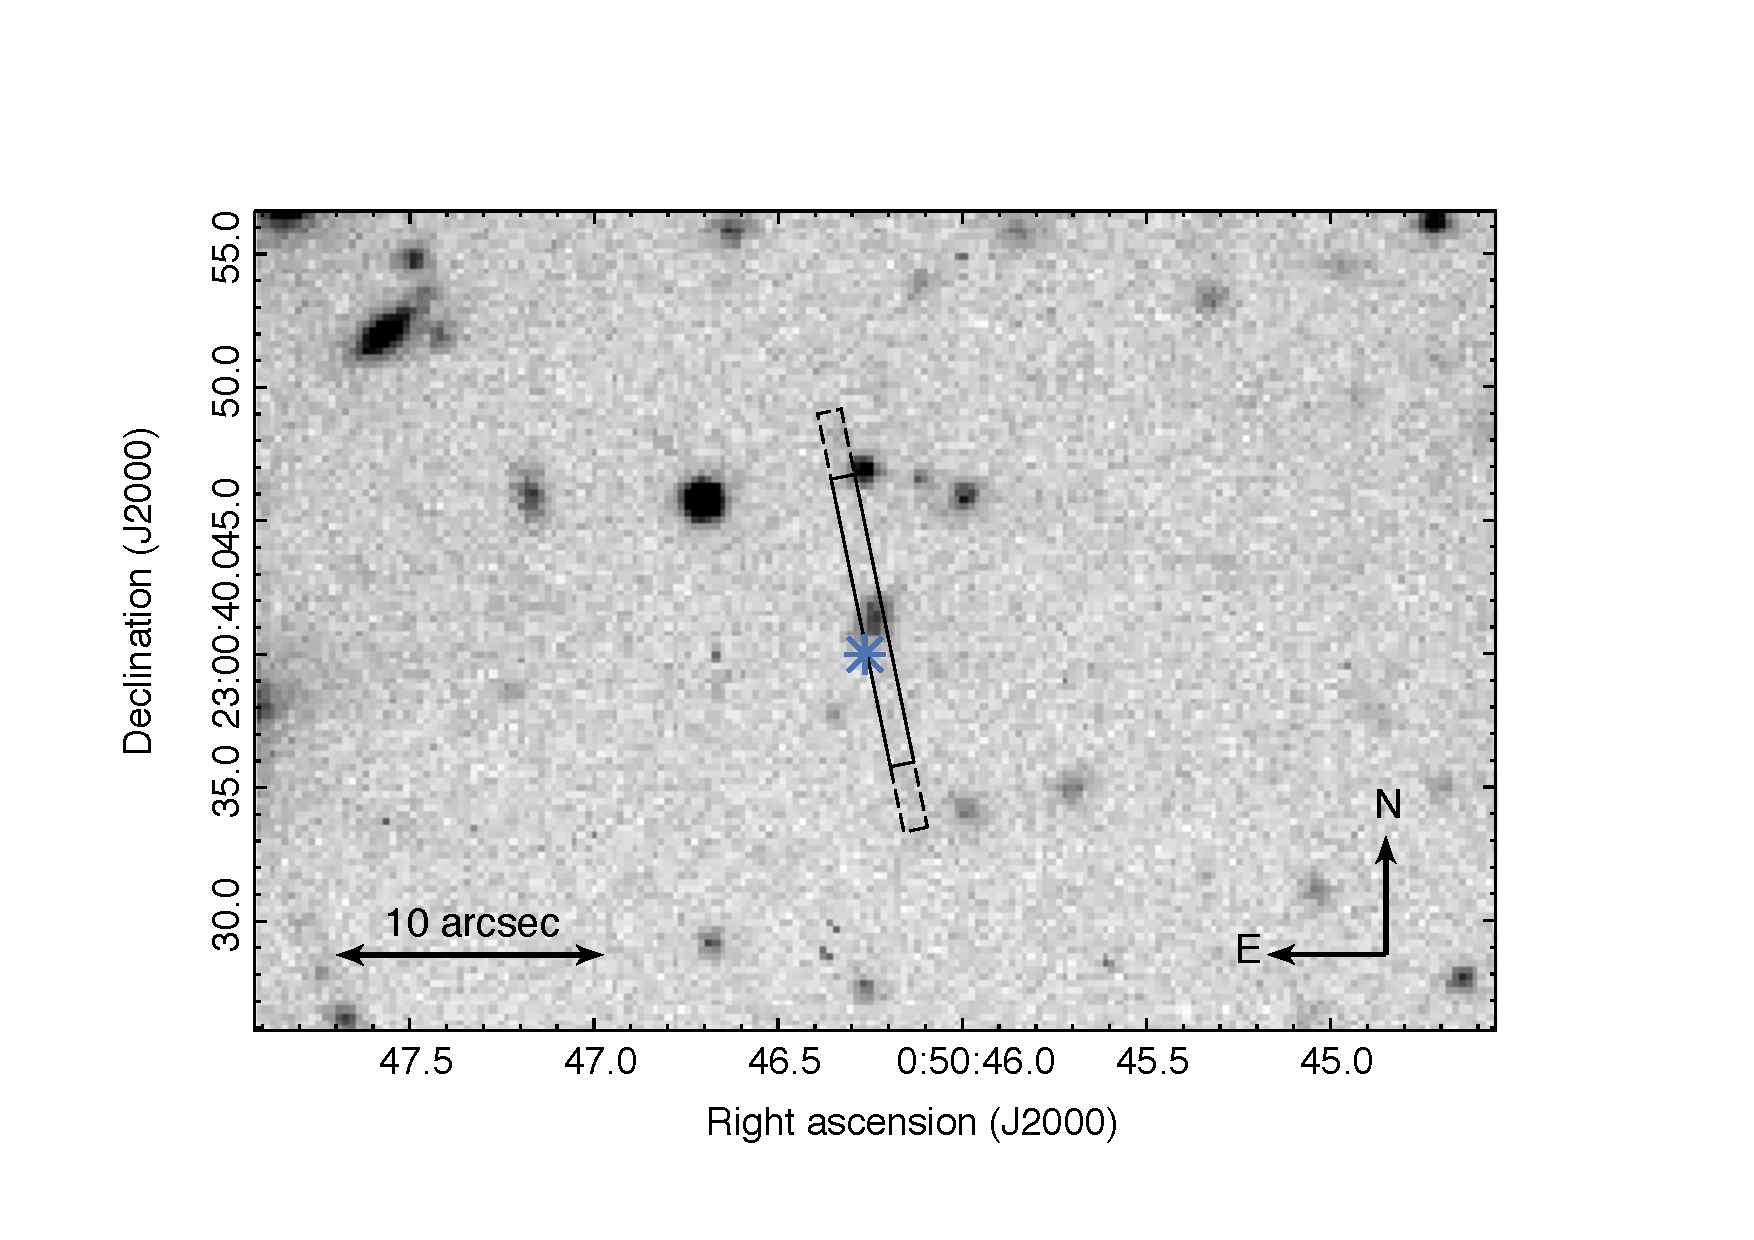
\includegraphics[width=9cm]{figures/GRB111117A_spec_obs.pdf}
	\caption{
	FORS2 $R$-band imaging of the field of GRB~111117A with the X-shooter slit
overlaid. The slit position represents 4 epochs of spectroscopic observations
taken at similar position angles. The corresponding photometry is shown in
Fig.~\ref{fig:SED}. The blue asterisk indicates the GRB position as derived
from the \emph{Chandra} observations in \citet{Sakamoto2013}.
	}
	\label{fig:spec_setup}
\end{figure}

%\begin{figure}
%	\centering
%	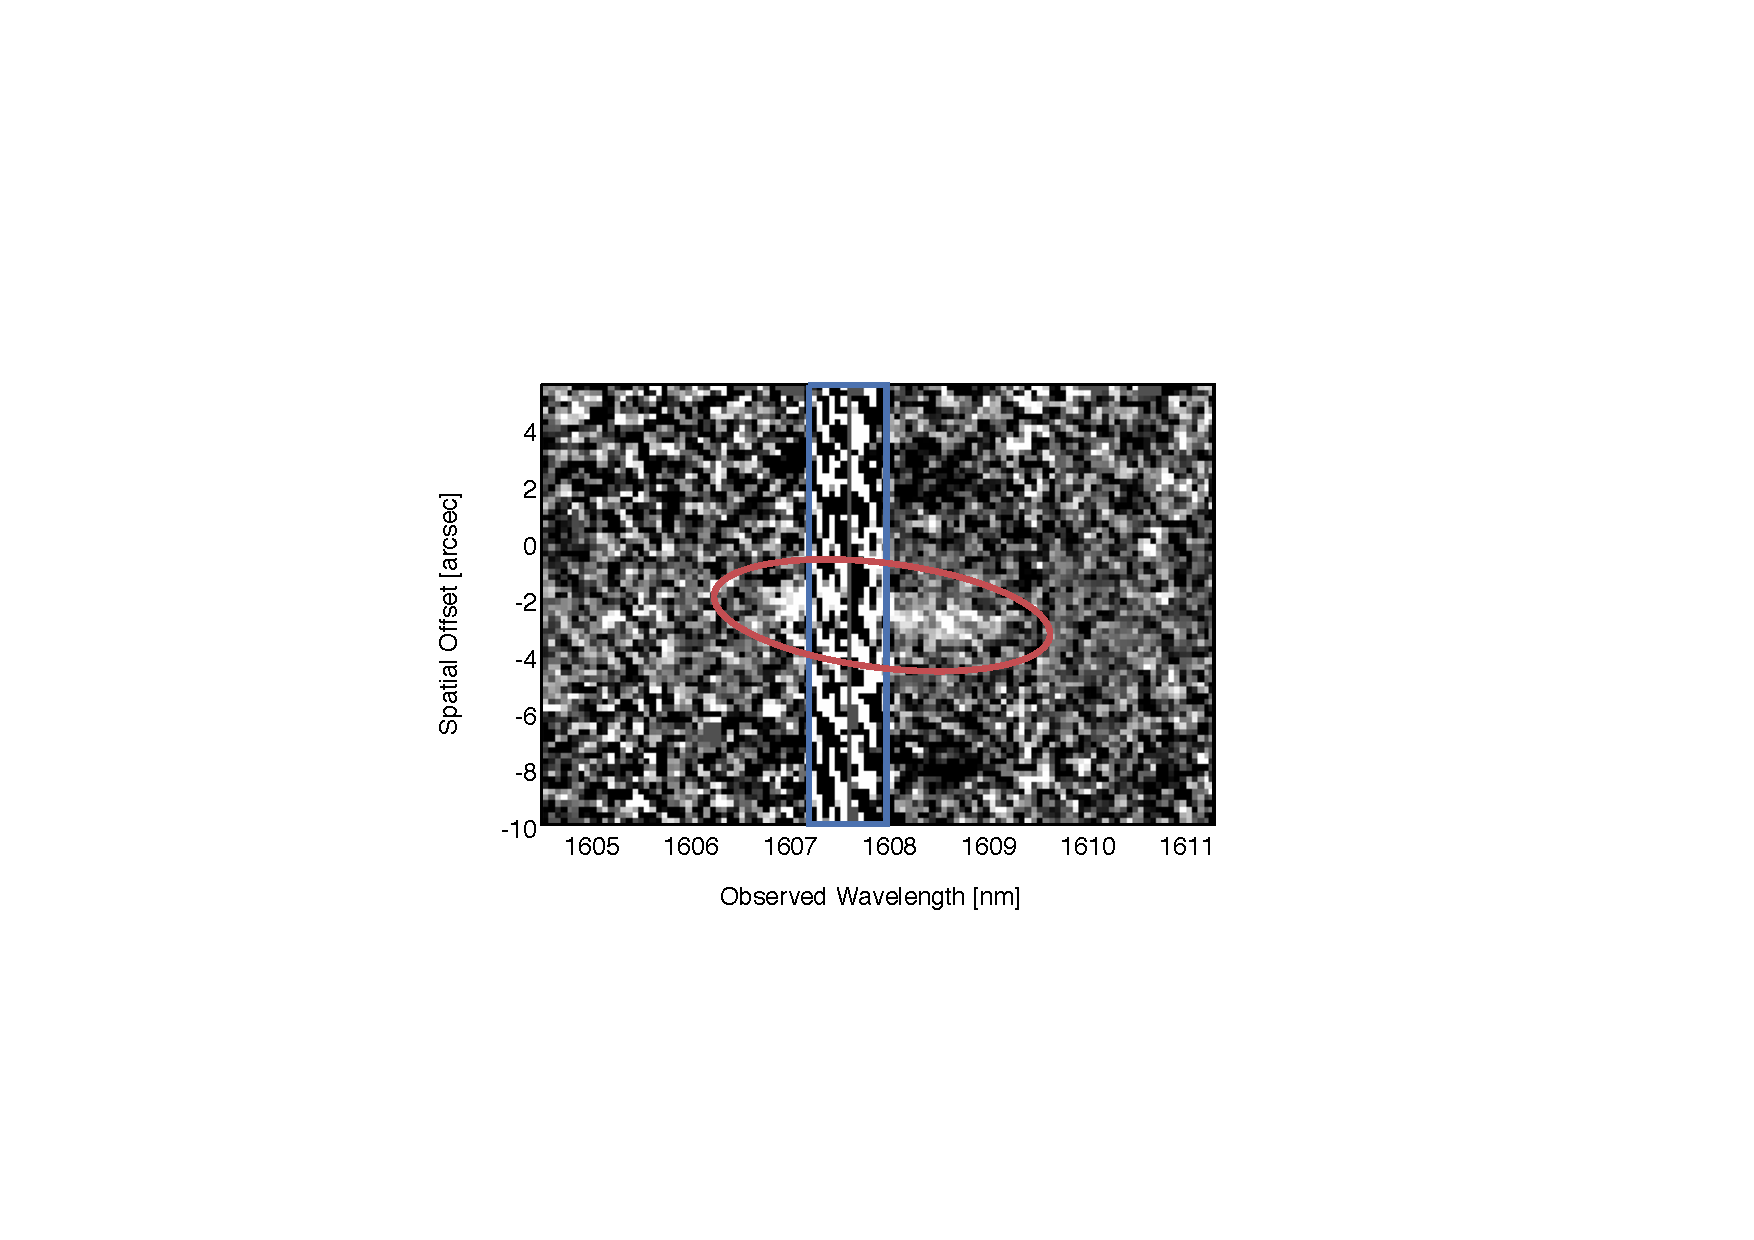
\includegraphics[width=9cm]{figures/OIII_img.pdf}
%	\caption{2D-image of the \oiii$\lambda$5007 emission line. The location of a bright skyline is marked by the blue box. The location of the emission line is indicated with the red ellipse. Because the host is observed in nodding-mode, negative images of the emission line appear on both sides in the spatial direction.}
%	\label{fig:line}
%\end{figure}


\begin{figure*}
	\centering
	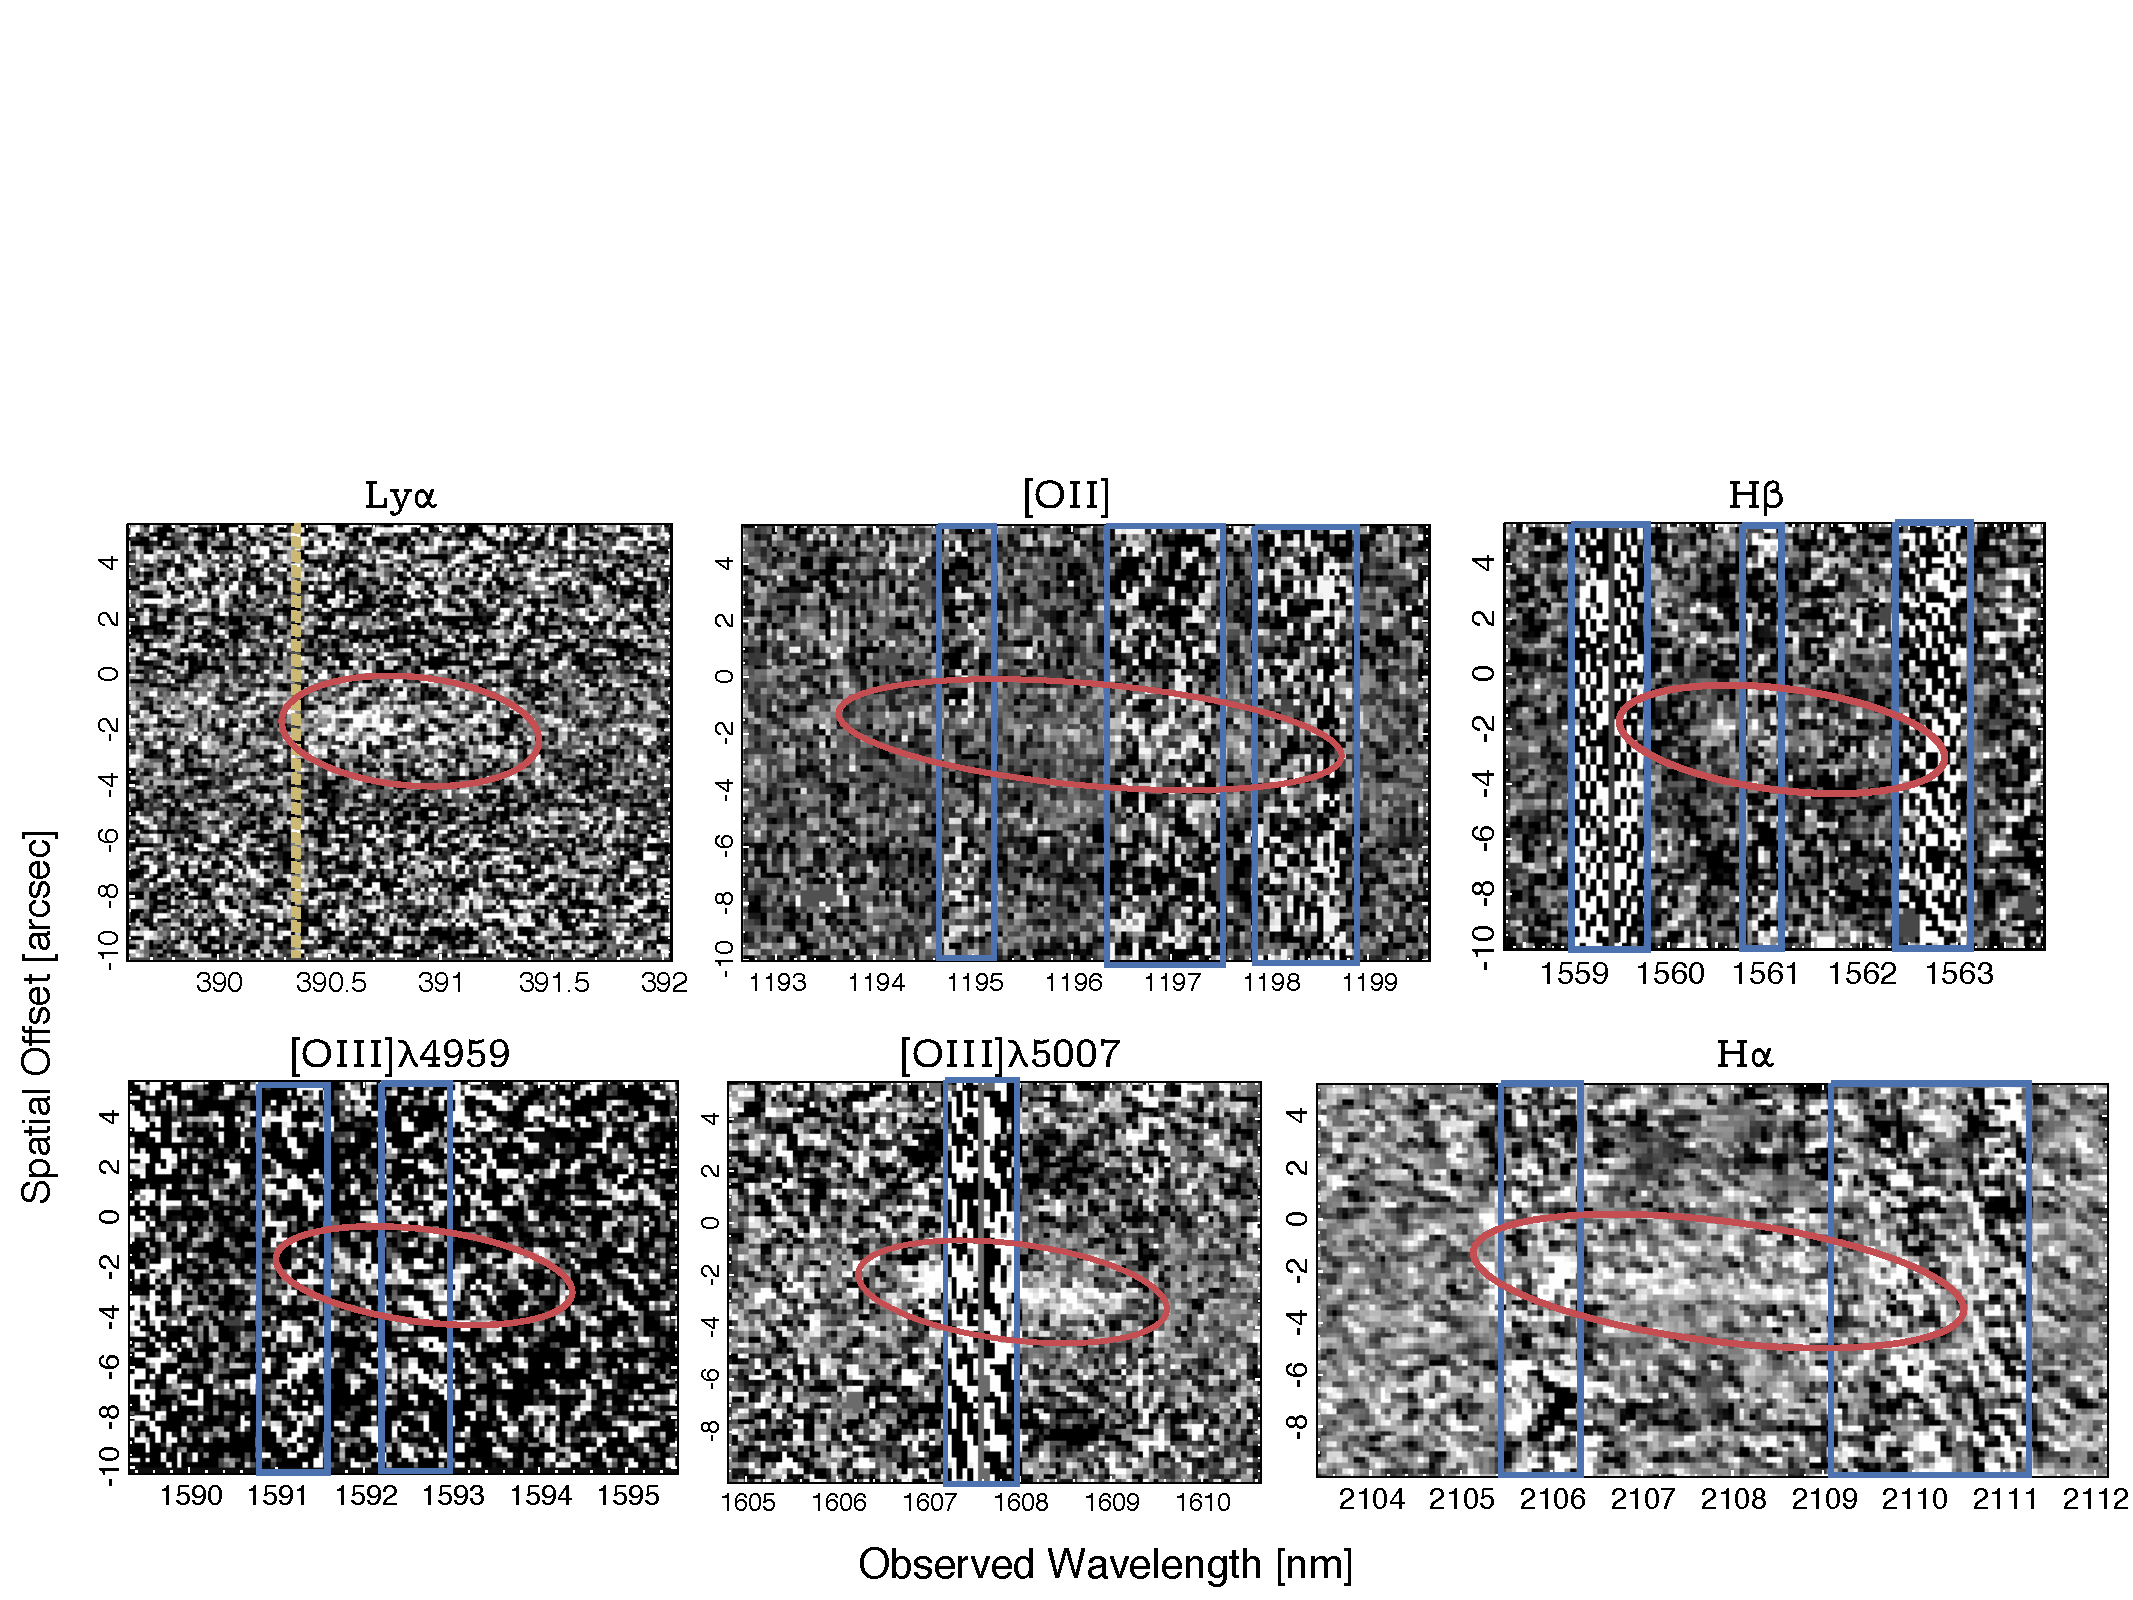
\includegraphics[width=18cm]{figures/grid.pdf}
	\caption{2D-images of the emission lines corresponding to \lya, \oii$\lambda$3727, \hb, \oiii$\lambda$4959, \oiii$\lambda$5007, and \ha. The location of bright skylines are marked by blue boxes. The locations of the emission lines are indicated with red ellipses. Because the host is observed in nodding-mode, negative images of the emission lines appear on both sides in the spatial direction. For the upper, left panel containing \lya, the systemic redshift position of \lya{} is marked by a yellow, vertical, dashed line. The red part of the \oii$\lambda$3727-doublet is affected by atmospheric absorption.}
	\label{fig:line}
\end{figure*}


\begin{figure*}
	\centering
	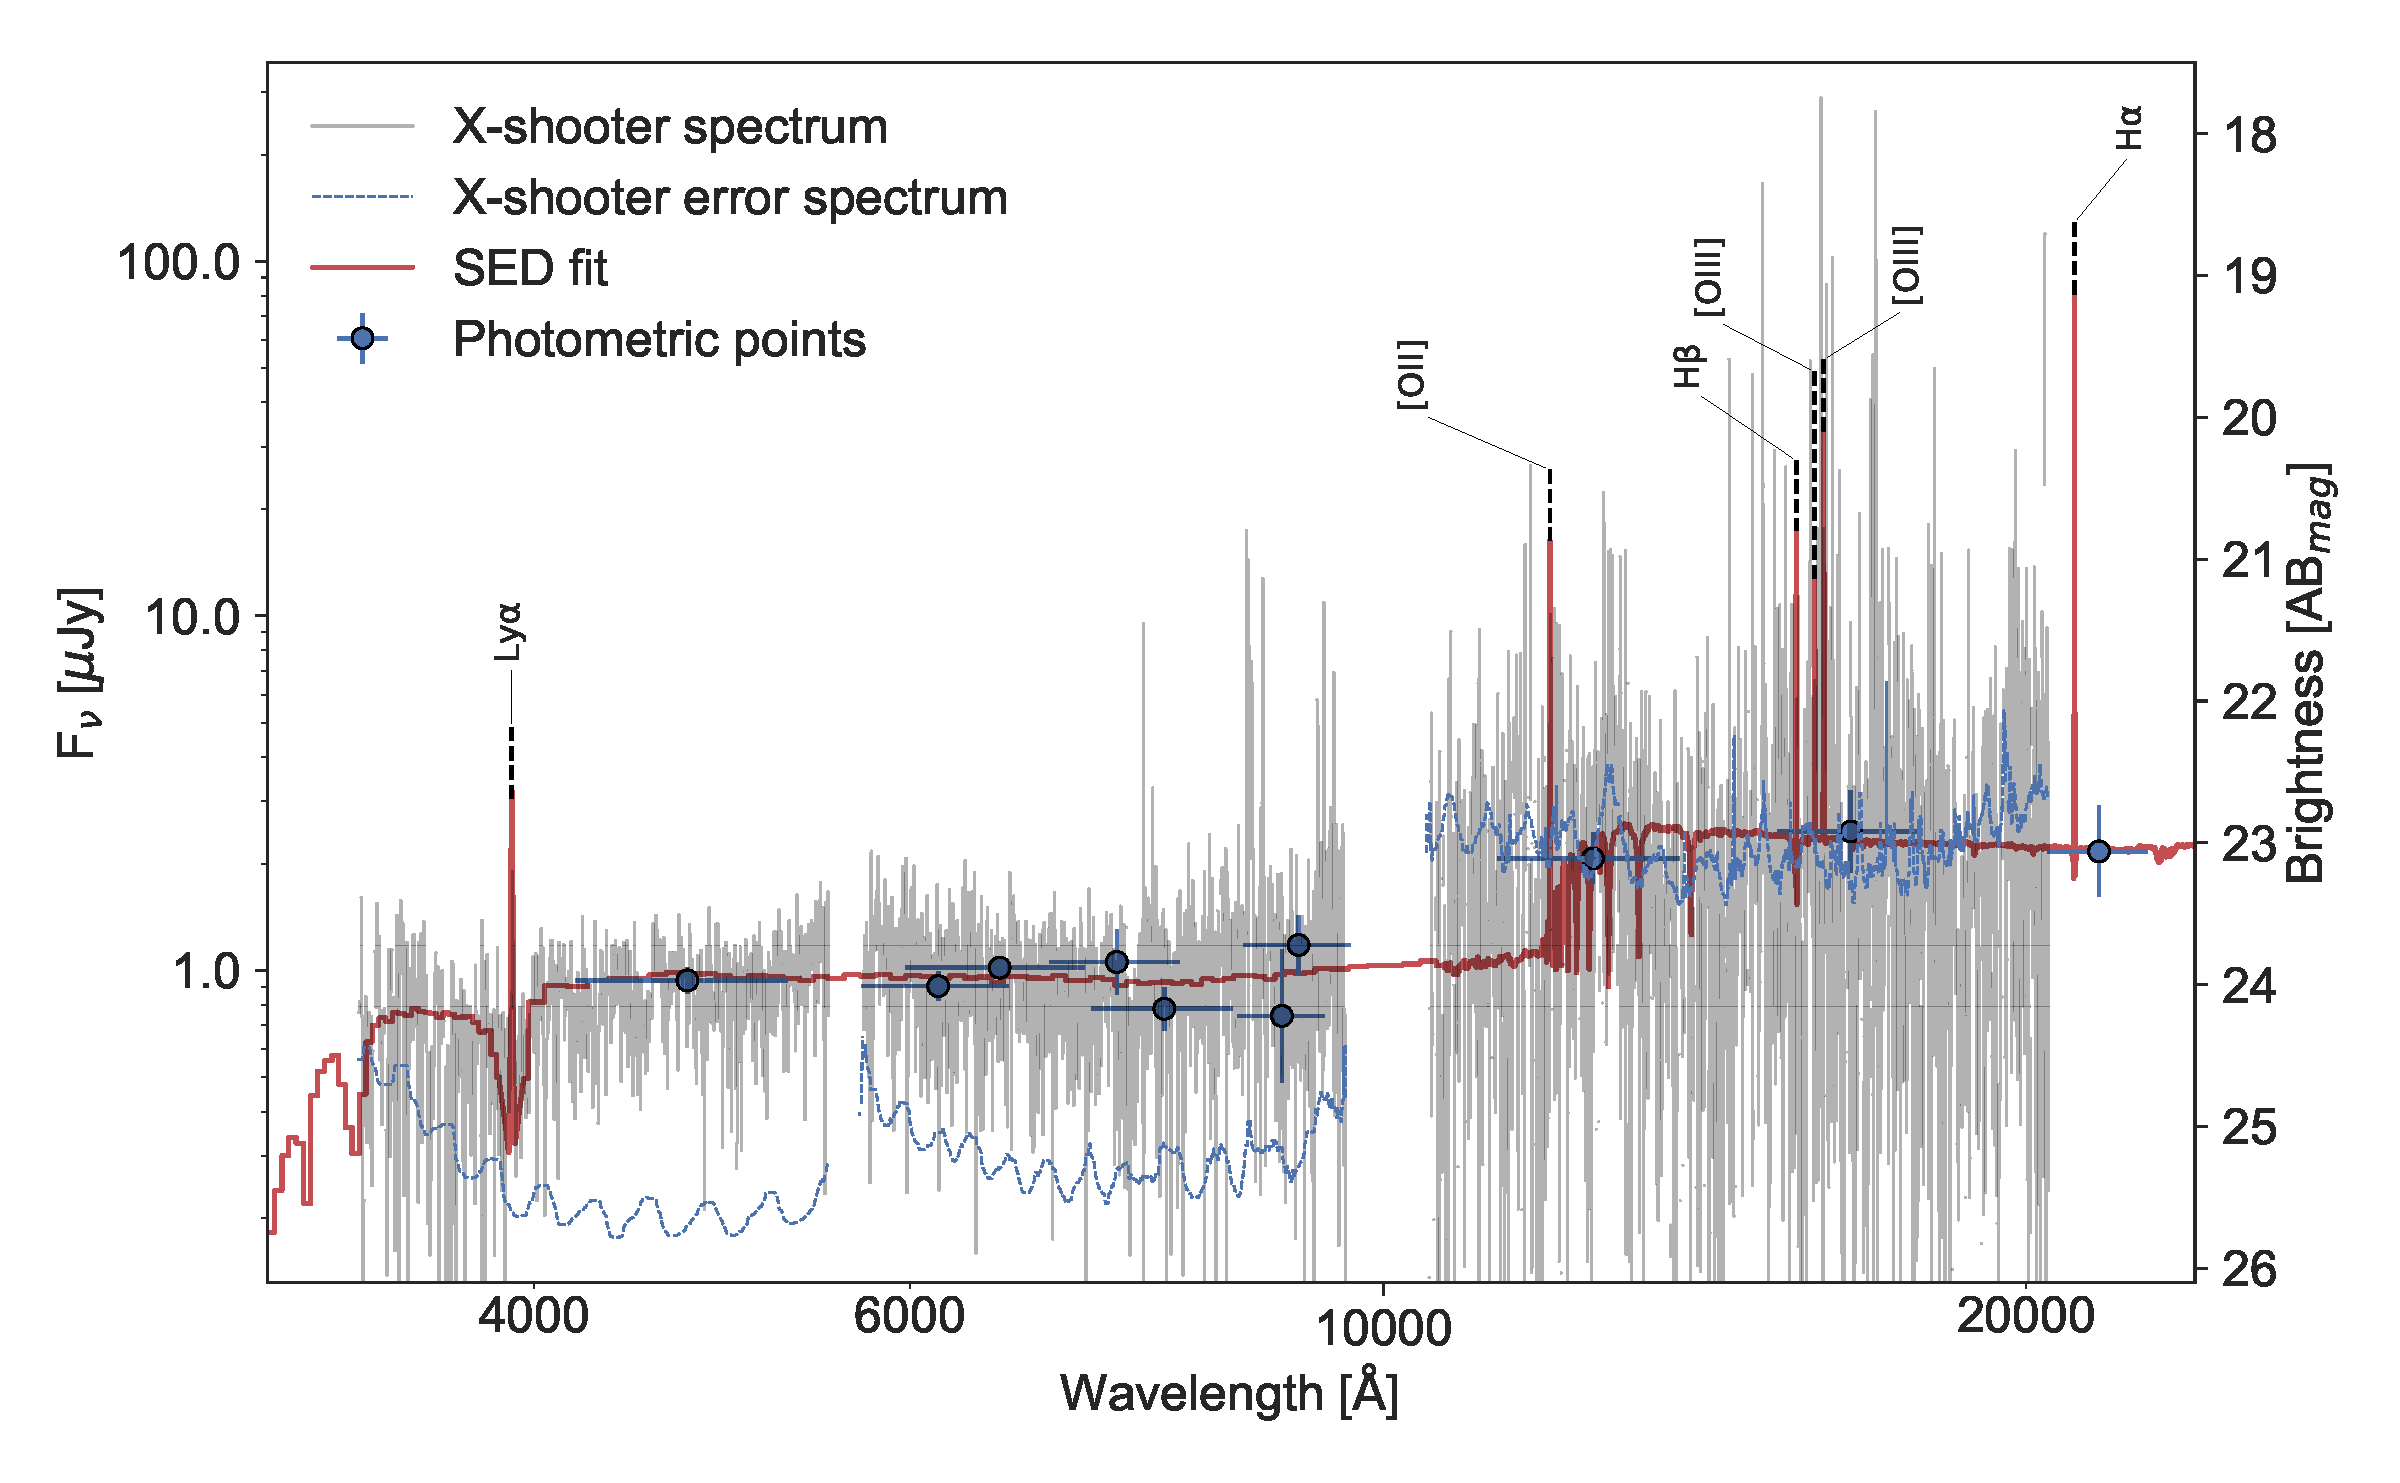
\includegraphics[width=16cm]{figures/SEDspecphot.pdf}
	\caption{Best-fit SED to the derived photometry. The detection of \lya{}  is predicted from the SED fit and confirmed by the spectroscopic observations. Overplotted in grey is the observed spectrum, binned by 6 \AA{} for presentation purposes. Slit losses has been corrected for based on the average seeing of the observations, as confirmed by the comparison with the photometry. The blue, dashed line is the corresponding error spectrum, smoothed for presentation purposes. The reason for the spectral gaps at 5500 \AA{} and 10000 \AA{} is from the merging of the arms.}
	\label{fig:SED}
\end{figure*}

Spectroscopic observations were carried out using the cross-dispersed echelle
spectrograph, VLT/X-shooter \citep{Vernet2011}, at four seperate epochs. The
burst was observed 38 hours after the Burst Alert Telescope (BAT) trigger under
ESO programme 088.A-0051 (PI: Fynbo) and again later under ESO programme
091.D-0904 (PI: Hjorth). Observations use a simple ABBA nodding pattern, with 5
\arcsec~nod throws. X-shooter covers the wavelength range from 3000~\AA{} to
24\,800~\AA{} (21\,000~\AA{} when the $K$-band blocking filter is used) across
three spectroscopic arms. We carried out the bias-correction, flat-fielding,
order tracing, wavelength calibration, rectification, and flux calibration using
the VLT/X-shooter pipeline version 2.8.4 \citep{Goldoni2006, Modigliani2010} run
in physical mode. Because the echelle orders are curved across each detector, a
rectification algorithm is employed which introduces correlations between
neighboring pixels. We select a pixel-scale of 0.2/0.2/0.6 \AA/pix for the
UVB/VIS/NIR arm to minimize the degree of correlation while conserving the
maximal resolution. The observations are combined and extracted using scripts
described in Selsing et al. 2017 (in prep.) and available
online\footnote{\url{https://github.com/jselsing/XSGRB_reduction_scripts}},
where the full spectral point spread function is modeled across each arm and
used for the optimal extraction algorithm \citep{Horne1986}. An overview of the
spectroscopic observations is given in Table~\ref{tab:spec_overview}, and the
slit position is shown in Fig.~\ref{fig:spec_setup}. Each of the epochs are
extracted individually and combined in a weighted fashion where the weight at
each pixel is chosen as median variance spectrum of the region surrounding that
pixel, thus avoiding to base the weight on the pixel variance. Slit-loss
correction has been applied on the combined spectrum based on the average seeing
of the observations. We show the extracted spectrum in Fig.~\ref{fig:SED}.

\begin{table*}[!ht]

	\centering
	\caption{Overview of the spectroscopic observations. ``JH'' in the slit width refers to observations where a $K$-band blocking filter has been used. The seeing is determined from the width of the spectral trace of a telluric standard star, observed close in time to the host observation. The spectral resolution, $R$, is measured from unresolved telluric absorption lines in the spectrum of the telluric standard star. \label{tab:spec_overview}}
	\begin{tabular}{cccccccc}
		\hline\hline
		{Observation epoch} &  \multicolumn{3}{c}{Exposure time (s)} & Slit width & Airmass & Seeing & $R$   \\ [1.5pt]
        \hline
		(UT) & UVB  & VIS & NIR &  (arcsec)   & {} & (arcsec)  & {VIS/NIR}  \\ [1.5pt]
		\hline
		2011-11-19 01:33 & 2 $\times$ 2400 & 2 $\times$ 2400 & 8 $\times$ 600 & 1.0/1.0/0.9 & 1.49 & 0.75 & 11600/6700 \\
        2013-07-15 09:02 & 2 $\times$ 1200 & 2 $\times$ 1200 & 8 $\times$ 300 & 1.0/1.0/0.9JH & 1.53 & 0.98 & 9600/8900 \\
        2013-08-03 07:37 & 2 $\times$ 1200 & 2 $\times$ 1200 & 8 $\times$ 300 & 1.0/1.0/0.9JH & 1.55 & 0.85 & 11400/11300 \\
        2013-08-03 08:34 & 2 $\times$ 1200 & 2 $\times$ 1200 & 8 $\times$ 300 & 1.0/1.0/0.9JH & 1.49 & 0.85 & 11400/11300 \\
		
		\hline\noalign{\smallskip}
		
	\end{tabular}

\end{table*}

We determine a redshift of $z = 2.211 \pm 0.001$ from the simultaneous detection
of emission lines belonging to \lya, \oii$\lambda$3727, \hb, \oiii$\lambda$4959,
\oiii$\lambda$5007, and \ha. \oii$\lambda$3727, \hb{}, and \oiii$\lambda$4959
are detected at low significance ($\sim$ 3-$\sigma$). The uncertainty on the
redshift is the standard deviation of independent measurements of the redshift
based on the individual line centroids (excluding \lya). We show cutouts of the
2D spectrum at the position of all the detected lines in Fig.~\ref{fig:line}. 
\ha{} is only visible in the first epoch due to the $K$-band blocking filter
used for the remaining observations. The nebular lines exhibit a spatial extent
of $\sim$ 1\farc5 and show significant velocity structure along the slit. A drop
in the continuum bluewards of the \lya{} line further supports the redshift. No
spectral evolution is observed across the epochs indicating that there is
negligible GRB afterglow contribution to the first epoch spectrum.

Using the luminosity of \ha, we can infer the SFR of the host
\citep{Kennicutt1998}. At the redshift of the GRB host, \ha{} is observed at
around 21\,000~\AA{} where the night sky is very bright. In addition, several
bright sky-lines are superposed on the line, making an accurate estimate of the
\ha~flux difficult. Due to their velocity structure, the lines exhibit clear
deviations from a Gaussian and given the low S/N of the spectra we do not
attempt any parametric fits. We instead obtain a limit on the SFR by numerically
integrating the part of \ha{} free of contamination and obtain $F_{\mathrm{H,X} \alpha} >
4.1 \times 10^{-17}~\mathrm{erg}~\mathrm{s}^{-1}~\mathrm{cm}^{-2}$. After
converting the \citet{Kennicutt1998} relation to a \citet{Chabrier2003} initial
mass function using the conversion factor from \citet{Madau2014}, we derive a
limit of $\mathrm{SFR} > 7 M_\odot$~yr$^{-1}$. We additionally obtain the \lya{} line
flux by numerically integrating the entire \lya{} line complex and obtain
$F_{\mathrm{Ly}\alpha} = (2.0 \pm 0.5) \times 10^{-17}~\mathrm{erg}~
\mathrm{s}^{-1}~\mathrm{cm}^{-2}$, where the error on the flux is found by
integrating the associated error spectrum over the same spectral region.

%Additionally, based on the width of \oiii, an aperture
%covering \ha is integrated over, where sky lines have been masked and
%interpolated over, using a synthetic sky spectrum \citep{Noll2012, Jones2013}.
%From the integrated \ha-line, we estimate SFR = $18 \pm 3$ M$_\odot$ yr$^{-1}$.
%The error on the SFR is derived from the integrated variance spectrum over the
%\ha-line and excluding the intrinsic scatter of the relation. 

From the SED-fit (Sect.~\ref{SED}) the host is constrained to contain very
little or no dust. Consistently, \lya{} is detected although its presence does
not exclude dust. Therefore we do not apply a dust-correction to the measured
\ha{} flux here. \oii{} is close to a region of strong telluric absorption,
which is why no SFR is inferred from this line.

The total extent of the lines in velocity space is $\sim$ 450 km s$^{-1}$. The line
profiles shows an asymmetric "double-horned" profile, indicating that we are
seeing a galaxy with a large degree of coherent rotational motion relative to
the line-of-sight. If we assume that we are viewing a spiral galaxy edge-on,
this is a measure of the rotational velocity of the gas. If we assume that the
spectral resolution and the turbulent width of the lines are negligible compared
to the rotational velocity, we can, based on the projected size of the source
and the width of the lines, put a constraint on the dynamical mass of the galaxy
\citep{DeBlok2014}. Based on the physical size along the slit and the velocity
width of \oiii$\lambda5007$, we infer $M_\text{dyn} \gtrsim 10^{10.8}$
$M_\odot$. Because we are viewing the host inclined at an angle relative to
edge-on and because the slit is not aligned along the long axis of the host,
this value is a lower limit. 

\subsection{Imaging observations and SED analysis} \label{SED}

In addition to the spectroscopy presented above, we imaged the field of
GRB~111117A in multiple broad-band filters using the VLT equipped with FORS2
($gRIz$ filters) and HAWK-I ($JHK_{\mathrm{s}}$ filters). These new data are
complemented by a re-analysis of some of the imaging used in
\citet{Margutti2012} and \citet{Sakamoto2013} that are available to us (GTC
$gri$-band, TNG $R$-band, and Gemini $z$-band). A log of the photometric
observations and measured brightnesses is given in
Table~\ref{tab:phot_overview}. Most data were taken long after the GRB had faded
when no afterglow contribution was present. Given the faintness of the afterglow
(see Sect. \ref{xray}, and \citealt{Cucchiara2011, Cenko2011}), we also expect
negligible contribution to the earliest epochs, which is confirmed by the
consistency between the two $g$-band measurements.

All data were reduced, analyzed and fitted in a similar manner as described in
detail in \citet{Kruhler2011a} and, more recently, in \citet{Schulze2016}. We
use our own \texttt{Python} and IRAF routines to perform a standard reduction
which includes bias/flat-field correction, de-fringing (where necessary),
sky-subtraction, and stacking of individual images. On the final reduced image
products, \texttt{DAOPHOT} \citep{Stetson1987} was used to derive the reported
photometry, where the size of the aperture was chosen to be 2\farc0. Because
image quality ranges from 0\farc6 - 1\farc7 and the galaxy major axis is $\sim$
1\farc, this ensures that, in all cases, the large majority of the flux is
collected and low-surface brightness light missed in the aperture will not
influence the measurement. This method sacrifices some S/N in the best seeing
cases for more reliable photometry across differing observing conditions.

Photometric calibration was fixed relative to field stars from the SDSS and
2MASS catalogs in the case of $griz$ and $JHK_{\mathrm{s}}$ filters,
respectively. For the $R$- and $I$-band photometry, we used the color
transformations of Lupton%
\footnote{\url{http://www.sdss3.org/dr8/algorithms/sdssUBVRITransform.php}}. We
convert all magnitudes into the AB system, and correct for a Galactic foreground
of $E_{B-V}=0.027~\mathrm{mag}$ \citep{Schlegel1998, Schlafly2011}.

Noteworthy is the discrepancy of both our new VLT/FORS2 photometry and the
re-analysis of the Gemini data compared to the $z$-band measurements of
\citet{Margutti2012} and \citet{Sakamoto2013}. Both of these authors report $z
\sim 23$, which is brighter than our measurement by $\sim 1.0$ mag, while data
taken in other filters are consistent within the errors. Visual inspection of
the Gemini image shows only a marginal detection of the host, which we report
here as a $\sim$ 2-$\sigma$ measurement. More conservatively, the 3-$\sigma$
upper limit for the Gemini image is $z > 24.06$. Objects of magnitude $z \sim
23$ are clearly seen and are significantly brighter than the GRB host galaxy.
The consistency between the deeper FORS2 $z$-band image and the upper limit
derived for the Gemini image lends credence to the inferred magnitudes presented
here, see Fig. \ref{fig:photplot}.

\begin{figure}
	\centering 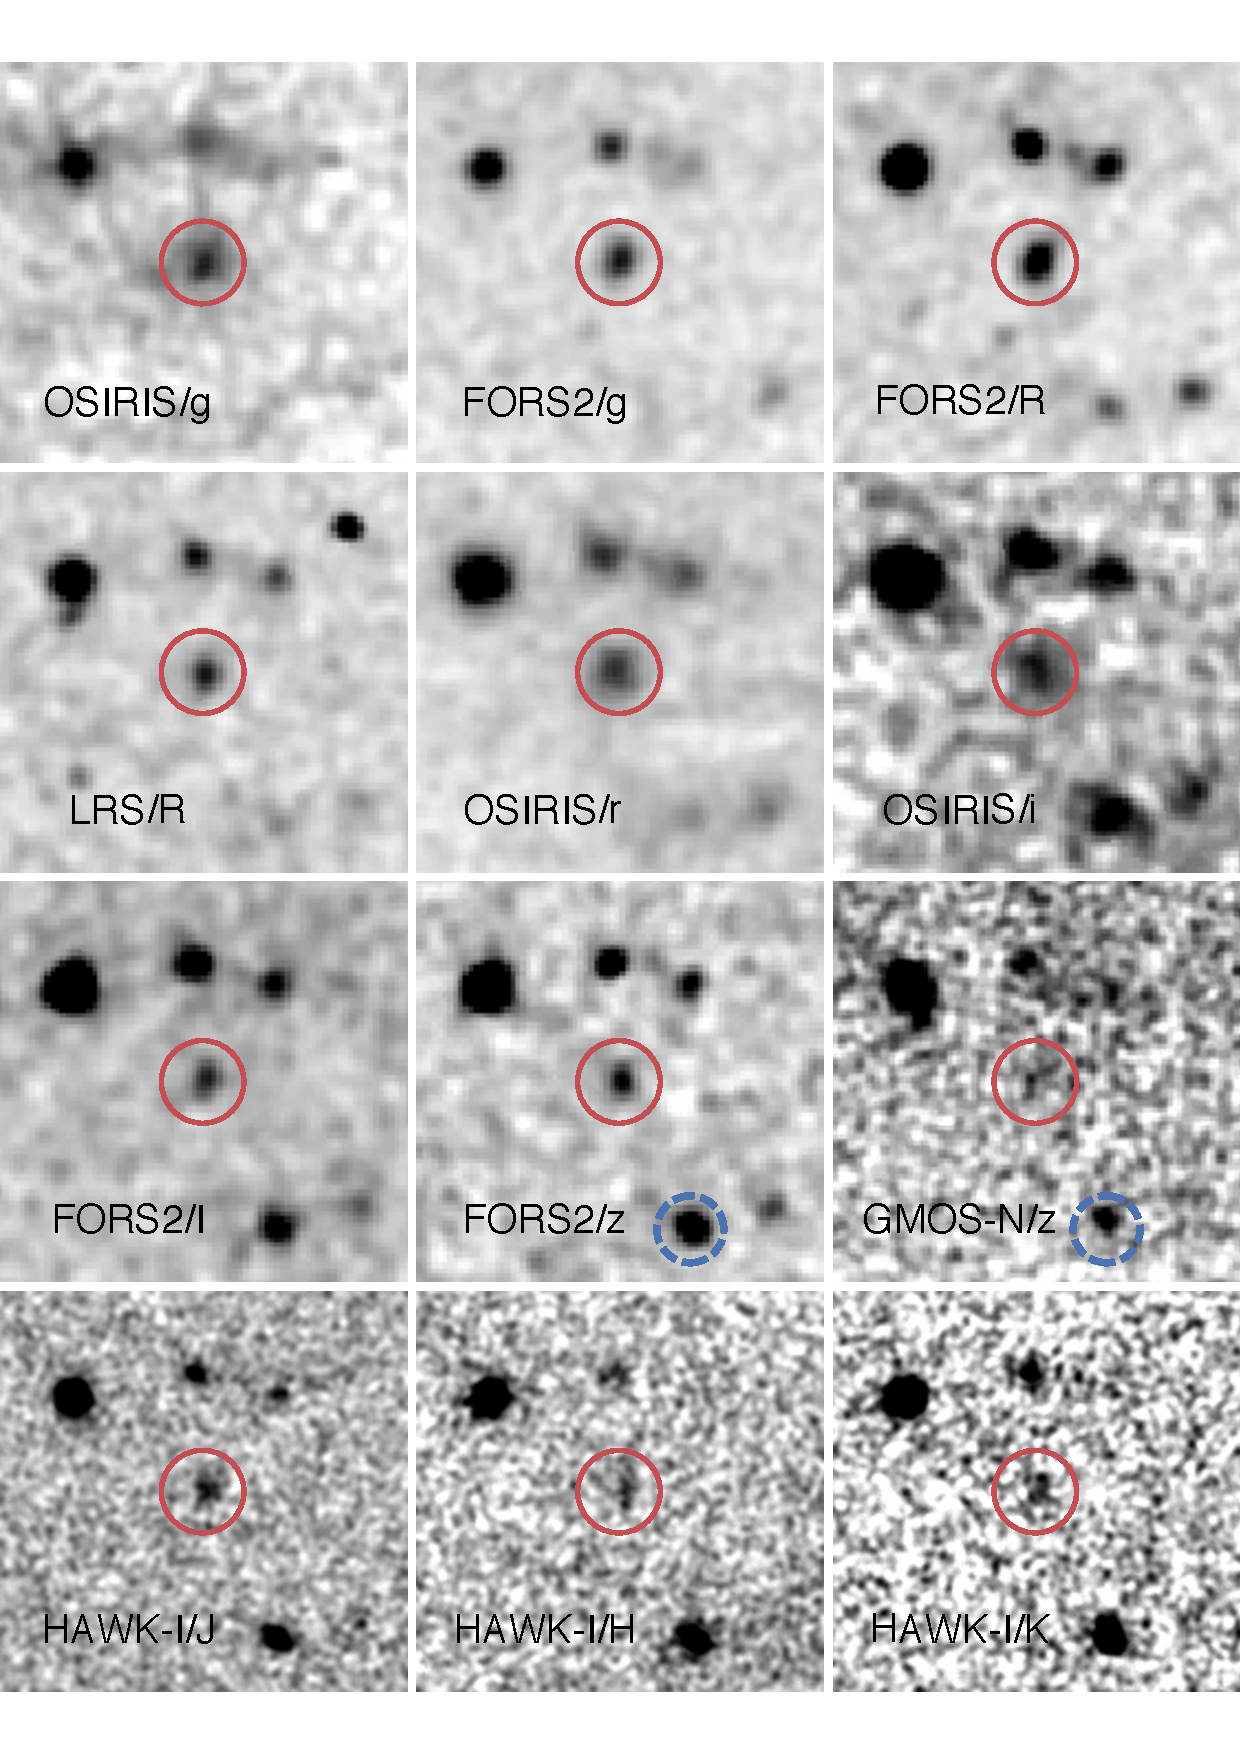
\includegraphics[width=9cm]{figures/photometry_mosaic.pdf}
\caption{Mosaic showing all used imaging. The host of GRB~111117A is marked by
	a red circle with a 2\farc0 radius. This is the same size as the aperture used
	for deriving the photometry. Each panel is 20\arcsec~in size, north is up, east
	is left. Worth noting is the relative depth of the GMOS-N and FORS2 $z$-band
	images. For reference, the object located to the south-east of the host and
	marked with a blue, dashed circle has an extinction corrected magnitude of
	$23.11 \pm 0.09$ ($23.10 \pm 0.18$) in the FORS2 (GMOS-N) $z$-band.}
\label{fig:photplot}
\end{figure}

\begin{table*}[!ht]

	\centering
	\caption{Overview of the photometric observations. \label{tab:phot_overview}}
	\begin{tabular}{ccccccc}
		\hline\hline
{Observation epoch} &  Exptime & Telescope/instrument & Filter & Airmass & Image quality & Host brightness\tablefootmark{a}  \\ [1.5pt]
        \hline
({UT}) & ({ks}) &    & {} & & (arcsec)  & (AB mag)  \\ [1.5pt]
		\hline
2013-08-30 07:43 & 1.45 & VLT/FORS2 & $g$ & 1.55 & 0.99 & $24.08\pm 0.09$ \\
2011-11-17 20:07 & 0.80 & GTC/OSIRIS & $g$ & 1.15 & 1.67 & $24.13\pm 0.09$ \\
2011-11-17 20:07 & 1.20 & GTC/OSIRIS & $r$ & 1.11 & 1.50 & $23.93\pm 0.08$ \\        
2013-07-17 08:37 & 1.45 & VLT/FORS2 & $R$ & 1.56 & 0.74 & $23.95\pm 0.06$ \\   
2011-11-28 21:10 & 3.60 & TNG/DOLORES & $R$ & 1.01 & 1.08 & $23.96\pm 0.13$ \\           
2011-11-17 20:07 & 0.36 & GTC/OSIRIS & $i$ & 1.08 & 1.50 & $23.89\pm 0.23$ \\   
2013-08-03 09:23 & 1.35 & VLT/FORS2 & $I$ & 1.54 & 0.93 & $24.22\pm 0.15$ \\           
2011-11-28 06:14 & 1.80 & Gemini/GMOS-N & $z$ & 1.01 & 0.84 & $24.24\pm 0.47$ \\  
2013-07-13 09:33 & 1.08 & VLT/FORS2 & $z$ & 1.49 & 0.63 & $23.76\pm 0.21$ \\             
2013-06-24 09:14 & 1.98 & VLT/HAWK-I & $J$ & 1.70 & 0.63 & $23.13\pm 0.18$ \\        
2013-06-27 09:21 & 1.68 & VLT/HAWK-I & $H$ & 1.63 & 0.91 & $22.94\pm 0.29$ \\   
2013-06-28 09:14 & 1.92 & VLT/HAWK-I & $K_\mathrm{s}$ & 1.65 & 0.76 & $23.07\pm 0.32$ \\   
\hline\noalign{\smallskip}
		
\end{tabular}

\tablefoot{
\tablefoottext{a}{All magnitudes are given in the AB system and are not corrected for the expected Galactic foreground extinction corresponding to a reddening of $E_{B-V}=0.027$\,mag.}}
\end{table*}

The multi-color SED is fit using the \citet{Bruzual2003} single stellar
population models (SSPs) based on a \citet{Chabrier2003} with initial mass
function in \emph{LePhare} \citep{Ilbert2006}, where the redshift is fixed to
the spectroscopic value of $z=2.211$. For the SED fitting, we create a grid
consisting of $\sim 10^6$  different galaxy templates with four metallicities
0.02, 0.2, 0.4, 1.0 $Z_{\odot}$, different ages, star-formation histories and
degrees of extinction. For every model, we calculate the likelihood, and create
a probability density function (PDF) for a given parameter by marginalizing over
the other parameters. We quote the median of the PDF as the best fit parameters
and the errors are the 16th and 84th percentiles of the PDFs \citep[e.g.
see][for details on the SED fitting procedure]{Schulze2016}.

The best fit model is an unreddened galaxy template. The inferred physical
parameters are the absolute magnitude ($M_B=-22.0\pm0.1$\,mag), the stellar mass
($\log(M_{\star}/M_\odot) = 9.9\pm0.2$), the stellar population age ($\tau =
0.5_{-0.3}^{+0.5}$ Gyr), and the star-formation rate
($\mathrm{SFR}_{\mathrm{SED}} = 11_{-4}^{+9}~M_\odot\,\mathrm{yr}^{-1}$). We
show the SED fit in Fig.~\ref{fig:SED}.

Without fixing the redshift to the spectroscopic value, using the revised
photometry from Table~\ref{tab:phot_overview}, the photometric redshift of the
galaxy is $z_{\mathrm{phot}}=2.04_{-0.21}^{+0.19}$, consistent with the
spectroscopic value at the 1-$\sigma$ confidence level. The large $i-z$ color
found in previous works was mistakenly interpreted as the 4000\,\AA{} break,
driving the galaxy photometric redshift to a lower, erroneous value.

%%%%%%%%%%%%%%%%%%%%%%%%%%%%%%%%%%%%%%%%%%%%%%%%%%%%%%%%%%%%%%%%%%%%%%%%%%%%
\subsection{X-ray temporal and spectral analysis}\label{xray}
%%%%%%%%%%%%%%%%%%%%%%%%%%%%%%%%%%%%%%%%%%%%%%%%%%%%%%%%%%%%%%%%%%%%%%%%%%%%

We retrieved the automated data products provided by the \textit{Swift}-XRT GRB
repository\footnote{\url{http://www.swift.ac.uk/xrt\_products/00507901}}
\citep{Evans2009}. 
The X-ray afterglow light curve can be fit with a single power-law decay with an
index $\alpha=1.27_{-0.10}^{+0.12}$. We performed a time-integrated spectral
analysis using data obtained in photon counting (PC) mode in the widest time epoch where
the $0.3-1.5\,\mathrm{keV}$ to $1.5-10\,\mathrm{keV}$ hardness ratio is constant
(namely, from $t-T_0 = 205$~s to $t-T_0 = 203.5$~ks, for a total of 29.1~ks of
data) to prevent spectral changes that can affect the X-ray column density
determination \citep{Kopac2012}. 
The obtained spectrum is well described by an absorbed power-law
model and the best-fit spectral parameters are a photon index of $2.1 \pm 0.4$ and
an intrinsic equivalent hydrogen column density $N_{\mathrm{H,X}}$ of $2.4_{-1.6}^{+2.4}
\times 10^{22}$~cm$^{-2}$ ($z=2.211$), assuming a solar abundance and a Galactic $N_{\mathrm{H,X}}$ in
the burst direction of $4.1 \times 10^{20}$~cm$^{-2}$ \citep{Willingale2013}.

A measure of the optical-to-X-ray flux ratio is parametrized in terms of the
"darkness"-parameter $\beta_\mathrm{OX} $ \citep{Jakobsson2004}. Using the optical
afterglow limits ($r' > 25.5$, 13.5 hr after the burst; \citealt{Cucchiara2011,
	Cenko2011}, the X-ray lightcurve can be interpolated and evaluated at the time
of the non-detection. We find $\beta_\mathrm{OX} < 0.79$, consistent with what was
reported in \citet{Sakamoto2013}.

%%%%%%%%%%%%%%%%%%%%%%%%%%%%%%%%%%%%%%%%%%%%%%%%%%%%%%%%%%%%%%%%%%%%%%%%%%%%
\section{Reinterpretation of the rest-frame properties}
%%%%%%%%%%%%%%%%%%%%%%%%%%%%%%%%%%%%%%%%%%%%%%%%%%%%%%%%%%%%%%%%%%%%%%%%%%%%

\citet{Margutti2012} find a projected offset between the host nucleus and the
GRB site of 1\farc25 $\pm$ 0\farc20 arcsec; \citet{Sakamoto2013}
find a similar value of 1\farc0 $\pm$ 0\farc20 arcsec. These correspond
to a projected physical offset at $z = 2.221$ of $10.6 \pm 1.7$ kpc and $8.5 \pm
1.7$ kpc respectively. Because the angular distance does not change
significantly between $z = 1.3$ and $z = 2.211$, all conclusions of
\citet{Margutti2012} and \citet{Sakamoto2013} relating to host offset are
unaffected.

%%%%%%%%%%%%%%%%%%%%%%%%%%%%%%%%%%%%%%%%%%%%%%%%%%%%%%%%%%%%%%%%%%%%%%%%%%%%
\subsection{Classification} \label{classification}
%%%%%%%%%%%%%%%%%%%%%%%%%%%%%%%%%%%%%%%%%%%%%%%%%%%%%%%%%%%%%%%%%%%%%%%%%%%%

Based on the BAT light-curve, $T_{90}=0.46$~s which is shorter than both the
prototypical 2~s \citep{Kouveliotou1993} and the $<0.8$~s suggested to also
exclude the shorter tail of the \textit{Swift}-observed lGRB population
\citep{Bromberg2012a}. Additionally, no signs of extended emission was found by
\citet{Sakamoto2013}. The spectral lag is $0.6 \pm2.4$ ms, consistent with zero.
As already pointed out by \citet{Margutti2012} and \citet{Sakamoto2013}, this is
typical of sGRBs, (however see also \citealt{Bernardini2015}). In conjunction
with the duration and the spectral hardness \citep{Sakamoto2011}, GRB~111117A is
thus securely classified as a sGRB. Because the observed classification
indicators, $T_{90}$ and hardness ratio, do not depend strongly on redshift
\citep{Littlejohns2013a}, the updated redshift does not change this designation.

The intrinsic luminosity is shown in the X-ray light curve (Fig.
\ref{fig:sxray_lightcurve}) and it is sub-luminous compared to the majority of
lGRBs. The inset in Fig. \ref{fig:sxray_lightcurve} shows the luminosity
distribution at 10 ks. The sub-samples comprise of 402 lGRBs, 31 sGRBs, and
GRB~111117A. The sample of lGRBs is from \citet{Evans2007, Evans2009} and the
sample of sGRBs is compiled from \citet{Kann2011, Berger2014} and
\citet{DAvanzo2014a}. The mean and the 1-$\sigma$ dispersions of the samples are
$\log(L_{\mathrm{lGRB}} / \mathrm{erg~s}^{-1}) = 46.59 \pm 0.87$ and
$\log(L_{\mathrm{sGRB}} / \mathrm{erg~s}^{-1})  = 44.96 \pm 0.94$ for the lGRB
and sGRB samples respectively. GRB~111117A had $\log(L / \mathrm{erg~s}^{-1}) =
44.95$ at 10 ks. This is very close to the peak of the sGRB luminosity
distribution at 10 ks, but an outlier from the lGRB distribution, further
supporting the short classification.

The separation of GRBs in two distinct classes based on their high-energy
observables points to an intrinsically different physical origin. LGRBs are
typically interpreted as collapsars \citep{MacFadyen1999} in which a single, massive
star undergoes gravitational collapse, where the currently preferred model for
sGRBs is the merger of two NSs \citep{Eichler1989, Nakar2007}.
\citet{Bromberg2013} investigated the degree to which high-energy observables of
the long and short GRB populations overlap and quantified the certainty in class
membership. According to \citet{Bromberg2013}, GRB~111117A has a $96_{-5}^{+3}$
percent probability of being a sGRB. Compared to two other sGRB candidates
at high redshift, GRB~060121 ($T_{90}=1.97 \pm 0.06$~s;
\citealt{DeUgartePostigo2006, Levan2006}) at $1.7 \lesssim z \lesssim 4.5$
($17_{-15}^{+14}$ per cent) and GRB~090426 ($T_{90}=1.28 \pm 0.09$~s;
\citealt{Antonelli2009, Levesque2010, Thone2011}) at $z = 2.609$ ($10_{-10}^{+15}$
per cent), the certainty in class membership for GRB~111117A is much higher.

Additionally, \citet{Horvath2010} classify both GRB~060121 and GRB~090426 as
intermediate-duration bursts. This comes from both events having very soft
spectra, as compared to the hard ones typically seen in sGRBs. Intermediate
bursts are very clearly related in their properties to lGRBs
\citep{DeUgartePostigo2011}, so they are unlikely to come from compact object
mergers. GRB~111117A is also securely classified as a sGRB according to the
\citet{Horvath2010} classification scheme.

A number of other GRBs are claimed to be short and at relatively high ($z \gtrsim 0.9$) redshift.
If we consider bursts with a probability of being short $f_{\mathrm{NC}} > 50$ per cent, according to the
\citet{Bromberg2013} classification scheme, 5 sGRB are found:
GRB~051210 at $z \sim 1.3$ ($f_{\mathrm{NC}} = 82_{-61}^{+10}$ per cent;
\citealt{Leibler2010}),
GRB~060801 at $z = 1.131$ ($f_{\mathrm{NC}} = 95_{-5}^{+3}$ per cent;
\citealt{Berger2007}),
GRB~070714 at $z = 0.923$ (no $f_{\mathrm{NC}}$ due to extended emission;
\citealt{Graham2009}),
GRB~090510 at $z = 0.903$ ($f_{\mathrm{NC}} = 97_{-29}^{+1}$ per cent;
\citealt{McBreen2010}), and
GRB~100117 at $z = 0.915$ ($f_{\mathrm{NC}} = 97_{-3}^{+1}$ per cent;
\citealt{Fong2011}). Although in individual cases a secure host association
(hence redshift determination) is uncertain, there does seem to be a number of sGRBs at $z
\sim 1$.

This securely makes GRB~111117A, by far, the highest redshift sGRB detected to
date. The redshift and classification of GRB~111117A imply that it occurred when
the universe was younger by $\sim$ 3 Gyr compared to any other securely
classified sGRB ever detected. If the merger of NSs is the primary agent for the
$r$-process element enrichment of the universe \citep{Goriely2011, Ji2016,
	Komiya2016}, this marks the earliest detection of this process.

\begin{figure}
	\centering
	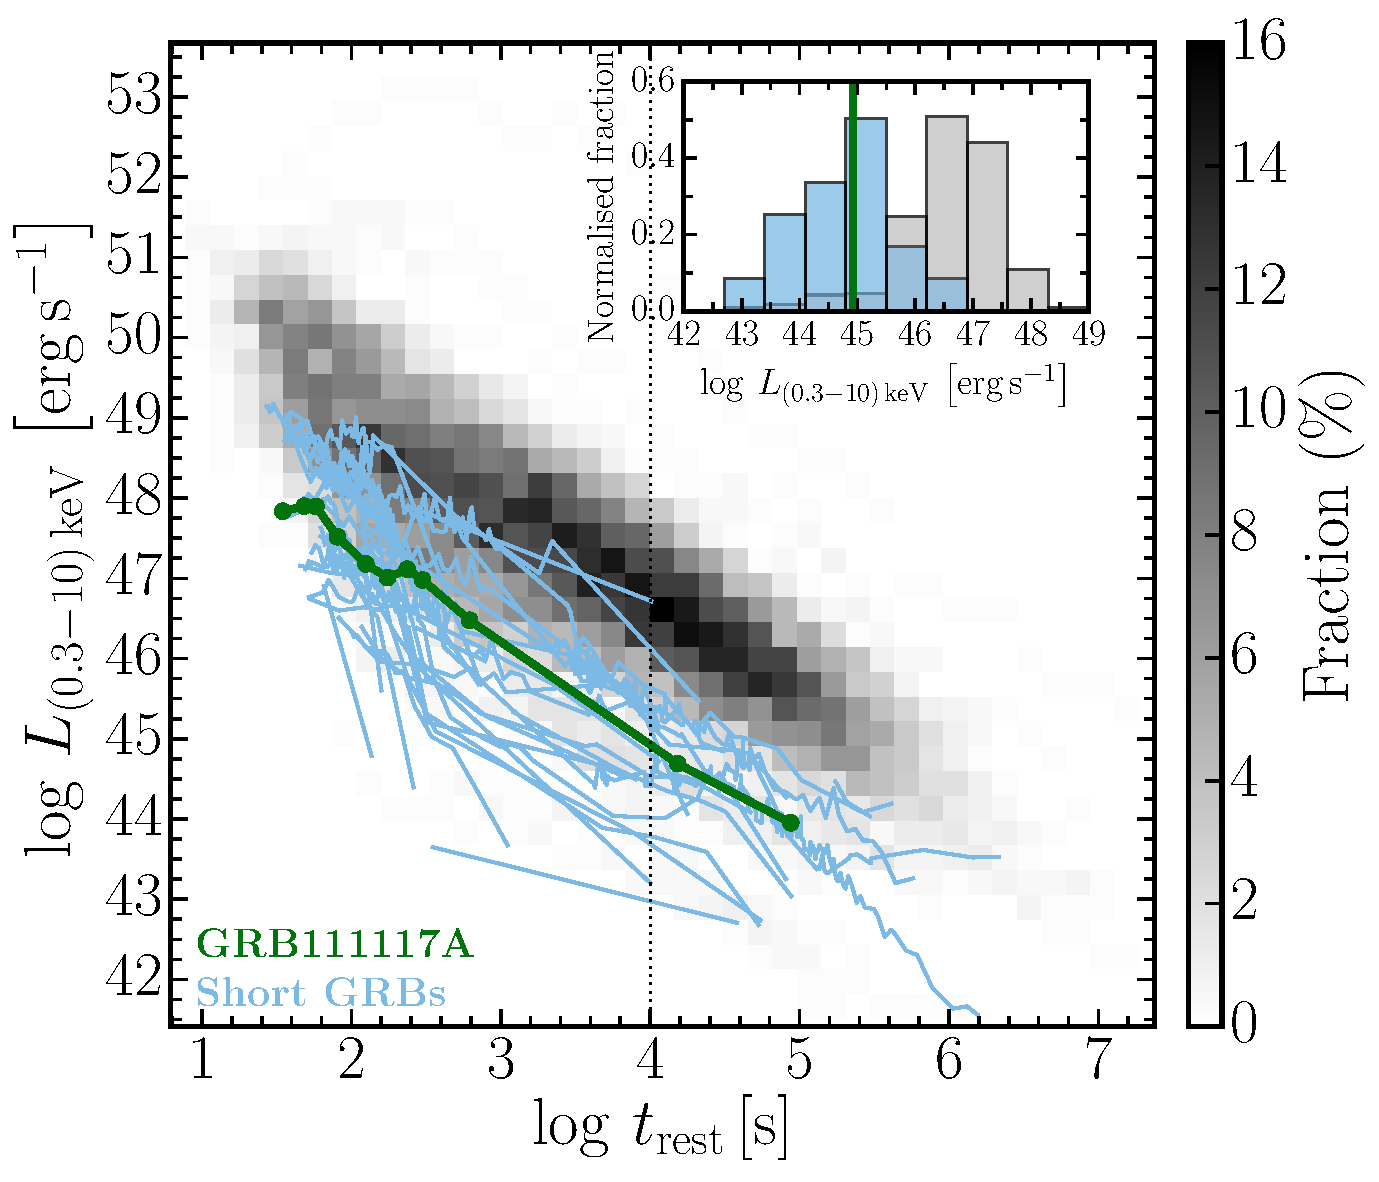
\includegraphics[width=9cm]{figures/XLC_111117A_rest.pdf}
	\caption{Rest-frame XRT lightcurve of GRB~111117A, compared to the general population of XRT lightcurves of GRBs. The grey shaded region is a compilation of long GRB lightcurves \citep{Evans2007, Evans2009} where the color represents density. The light blue lines are sGRB lightcurves from bursts with duration of $T_{90} \lesssim 2$ s and those that were classified as short in \citet{Kann2011, Berger2014, DAvanzo2014a}. The thick green line is GRB~111117A. Despite the remarkably high redshift, the luminosity is comparable to the bulk of the short burst population and subluminous compared to the lGRB population. The insert shows the X-ray luminosity distributions of sGRBs and lGRBs at 10 ks, indicated by the vertical dashed line in the main panel.}
	\label{fig:sxray_lightcurve}
\end{figure}

%%%%%%%%%%%%%%%%%%%%%%%%%%%%%%%%%%%%%%%%%%%%%%%%%%%%%%%%%%%%%%%%%%%%%%%%%%%%
\subsection{Rest-frame $N_\mathrm{H,X}$ } \label{restnH}
%%%%%%%%%%%%%%%%%%%%%%%%%%%%%%%%%%%%%%%%%%%%%%%%%%%%%%%%%%%%%%%%%%%%%%%%%%%%

We show the recalculated hydrogen equivalent X-ray derived column density,
$N_\mathrm{H,X}$, in Fig.~\ref{fig:NH_z} where we compare with the distributions
of complete samples of both long and short GRBs. The lGRB sample is from
\citet{Arcodia2016} and the sGRB sample is from \citet{DAvanzo2014a}. From the
sGRB sample of \citet{DAvanzo2014a} we have excluded GRB~090426 which does
likely not belong in a short sample as highlighted in Sect.
\ref{classification}. Both comparison samples infer $N_\mathrm{H,X}$  over the
largest temporal interval of constant hardness ratio to exclude spectral changes
that can affect the X-ray derived column density. The 17 (5) of the 99 (15) long
(short) GRBs which do not have measured redshifts have been excluded from our
analysis.

GRB~111117A occupies a unique position in Fig.~\ref{fig:NH_z} with the highest
$N_\mathrm{H,X}$ and highest redshift of all sGRBs. The short sample, excluding
GRB~111117A, is located at low redshift ($z < 1$) and is found to populate a
column density environment similar to that of lGRBs at comparable redshifts
\citep{DAvanzo2014a}. The inferred hydrogen column density for GRB~111117A seems
to follow the trend with increasing $N_\mathrm{H,X}$ as a function of redshift as found for
the lGRB afterglows \citep{Campana2010, Starling2013, Arcodia2016}. This is
related to what is found by \citet{Kopac2012, Margutti2013}, that $N_\mathrm{H,X}$ seems to
be comparable for long and short GRBs when compared at similar redshifts.

The redshift evolution of $N_\mathrm{H,X}$ in the hosts of lGRBs is not
reproduced by \citet{Buchner2017}, using a different $N_\mathrm{H,X}$ inference
methodology. Instead a correlation between $N_\mathrm{H,X}$ and host stellar
mass is suggested. Assuming that the different $N_\mathrm{H,X}$-fitting
methodologies yield comparable results, GRB~111117A has a larger
$N_\mathrm{H,X}$ compared to the relation suggested by \citet{Buchner2017} by
more than the intrinsic scatter, although some lGRB hosts populate a similar
region in the $N_\mathrm{H,X}$-$M_\star$ relation.
% Additionally, for lGRBs,
%$N_\mathrm{H,X}$ correlates with the surface luminosity at the explosion site
%\citep{Lyman2017}.

The large offset of GRB\,111117A relative to the host center derived in
\citet{Margutti2012} and \citet{Sakamoto2013} is difficult to reconcile with
galaxy-scale gas being the source of the X-ray absorption. Along with the low
dust content of the host, the large offset from the host center indicates that
the high $N_\mathrm{H,X}$ arises because the density in the GRB surroundings is
high (or possibly because the light from the afterglow transverses localized
regions of dense gas), see for example,
\citep[e.g.][]{Watson2013, Krongold2013}. Alternatively, it has been
hypothesised that a significant contribution to the observed X-ray
$N_\mathrm{H,X}$ could come from the diffuse intergalactic medium and the
intervening systems along the line of sight of the GRB \citep{Campana2012,
	Arcodia2016}, although see \citep{Watson2013, Krongold2013}.

Even assuming a low dust-to-metals ratio as typically observed in long GRB
afterglow sightlines \citep{Galama2001, Schady2010, Covino2013}, the
$N_\mathrm{H,X}$ value derived from the X-ray spectrum corresponds to
significant extinction along the afterglow line of sight ($A_V \gtrsim 1$~mag),
which is contrasted to the absence of dust found from the SED fit and supported
by the detection of \lya{}. Such a discrepancy between the extinction derived
from the GRB afterglow and the one obtained using galaxy-wide measures has also
been observed occasionally for lGRBs \citep{Perley2013a}. For the one sGRB where
both parameters were measured (GRB~130603B; \citealt{DeUgartePostigo2014b}),
they were found to be consistent with $A_V \sim 1$~mag.

The lack of optical detection is also consistent with a high column along the
GRB line of sight, as dust extinction could contribute to the optical faintness.
On the contrary, its X-ray afterglow flux lies within the expected distribution
given its gamma-ray fluence \citep{DAvanzo2014a}. This is not unexpected, as the
X-ray flux is independent of the surrounding medium density \citep{Freedman2001,
	Berger2003, Nysewander2009}.

\begin{figure}
	\centering 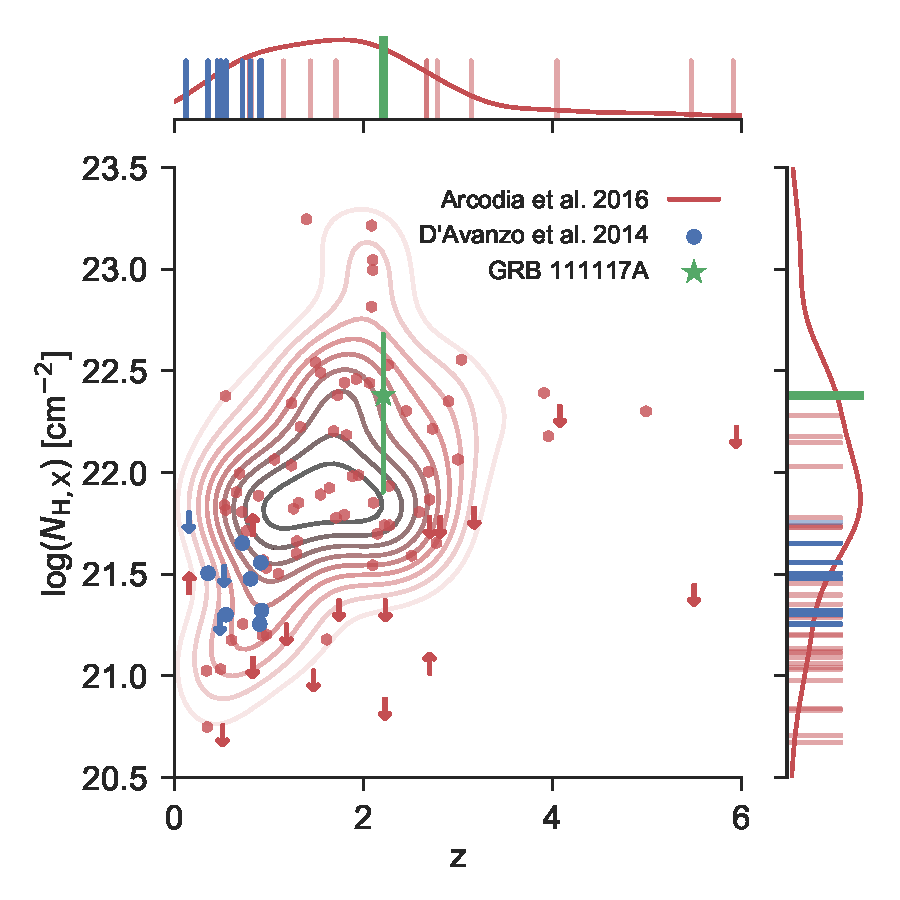
\includegraphics[width=9cm]{figures/NH_z.pdf} \caption{Rest frame,
	X-ray derived equivalent hydrogen column density of GRB~111117A compared to
	complete samples of both long and short populations of GRBs. The sample of
	lGRBs from \citet{Arcodia2016} is shown in red, where detections are also shown
	with a kernel density estimate of the points and the limits on $N_\mathrm{H,X}$
	are shown with arrows. The complete sample of sGRB by \citet{DAvanzo2014a} is
	shown in blue, where again the limits are indicated by arrows. Marginalizations
	over both axes are shown on the right and on the top of the plot, where the
	limits are shown as semi-transparent bars and detections as solid ones. The red
	curves in the marginalization plots are again the kernel density estimates of
	the \citet{Arcodia2016} sample.} \label{fig:NH_z}
\end{figure}


%%%%%%%%%%%%%%%%%%%%%%%%%%%%%%%%%%%%%%%%%%%%%%%%%%%%%%%%%%%%%%%%%%%%%%%%%%%%
\subsection{Host galaxy}
%%%%%%%%%%%%%%%%%%%%%%%%%%%%%%%%%%%%%%%%%%%%%%%%%%%%%%%%%%%%%%%%%%%%%%%%%%%%

Because of the secure host association, GRB~111117A does not belong to the
hostless class of sGRBs \citep{Berger2010a} and because the host exhibits
emission lines this is indicative of a population of relatively young stars.
Like the majority of sGRBs \citep{Fong2013b}, the host of GRB~111117A is
therefore a late-type galaxy and is entirely consistent in terms of stellar mass
and stellar age with the general population of sGRB hosts ($\left\langle M _*
\right\rangle = 10^{10.1} M_{\odot}$ and $\left\langle \tau _* \right\rangle =
0.3 $~Gyr; \citealt{Leibler2010}). Being a late-type host, both the stellar mass
and sSFR are entirely within the range expected for the hosts of sGRBs
\citep{Behroozi2014}. Our constraint on the dynamical mass is also well
accommodated by the expected sGRB host halo mass \citep{Behroozi2014}.

The SFR is $\sim$1 order of magnitude higher than the typical SFR for sGRB host
galaxies \citep{Berger2014} and more similar to the SFR found in the hosts of
lGRBs at a corresponding redshift \citep{Kruhler2015}. Only two hosts in the
sample of short GRBs compiled by \citet{Berger2014} have a more vigorous star
formation, placing it is in the very upper end of the star formation
distribution. The cosmic SFR evolution of the universe likely plays a role due
to the proximity of GRB~111117A to the peak of cosmic SFR \citep{Madau2014}.
The high SFR is partly a selection effect, because a less star forming galaxy
would exhibit weaker emission lines, thus making the redshift harder to
determine. Additionally, it is natural to expect some evolution in the hosts of
sGRBs with redshift as illustrated for $N_\mathrm{H,X}$ in Sect.~\ref{restnH}.

The simultaneus detection of \lya{} and \ha{} allows us to put constraints of
the escape fraction of \lya{}, $f_{\mathrm{esc}}$(\lya). Using the intrinsic
ratio between \ha{} and \lya{}, assuming case B recombination
\citep{Brocklehurst1971}, and the measured fluxes from the spectrum, we find
$f_{\mathrm{esc}}$(\lya)$ < 0.06$. While the $f_{\mathrm{esc}}$(\lya) scales
with the dust column \citep{Hayes2011}, the resonant scattering of
\lya{}-photons with neutral hydrogen makes the effective path length of \lya{}
longer than for \ha{} \citep{Atek2009}. This makes $f_{\mathrm{esc}}$(\lya) an
unreliable proxy for dust column, especially at low dust columns
\citep{Atek2014} where the geometry and dynamics of the \hi{} within the galaxy
will affect the \lya{} path the most. The $f_{\mathrm{esc}}$(\lya) inferred for
the host is entirely consistent with what is found for field galaxies with
similar properties \citep{Oyarzun2017}. The same authors also find that \lya{}
emitting galaxies have mostly little dust, consistent with what inferred from
the SED fit(see Sect. \ref{SED}). The centroid of the Ly$\alpha$ emission is
found to be redshifted by $\sim$~$240\pm 90$~km~s$^{-1}$ with respect to
systemic, which is similar to what is found for long GRB hosts
\citep{Milvang-Jensen2012a} and Lyman break galaxies \citep{Shapley2003a} in
which the outflow is attributed to star formation.

%%%%%%%%%%%%%%%%%%%%%%%%%%%%%%%%%%%%%%%%%%%%%%%%%%%%%%%%%%%%%%%%%%%%%%%%%%%%
\section{Implications for the redshift distribution of sGRBs}
%%%%%%%%%%%%%%%%%%%%%%%%%%%%%%%%%%%%%%%%%%%%%%%%%%%%%%%%%%%%%%%%%%%%%%%%%%%%


The redshift distribution of GRBs is a powerful informant on both the conditions
which drive the formation of these events, but also on the potential influence
these cosmic explosions have on the evolution of the universe. Due to the
elevated brightness of lGRBs compared to sGRBs \citep{Berger2014} and their
tendency to be associated with the star-forming and therefore dense regions in
their hosts \citep{Fruchter2006, Lyman2017}, the redshifts of lGRBs are easier
to measure than for sGRB counterparts, where only a single burst has a redshift
measurement from the GRB afterglow \citep{Cucchiara2013, DeUgartePostigo2014b}.
Correspondingly, the redshift distribution of sGRBs is still substantially
unconstrained compared to that of lGRBs \citep[e.g., see][]{Jakobsson2012a,
	DAvanzo2015, Perley2016d}.

A single sGRB at high redshift does little in terms of constraining the redshift
distribution of sGRBs. In particular, other sGRB host redshifts could have been
missed because their hosts are intrinsically fainter and thus the high redshift
of GRB~111117A is only measured due to the brightness of its host.
\citet{Berger2014} compiled a sample of sGRB host luminosities, normalized by
the characteristic galaxy luminosity at their respective redshift,
$L_B/L^{\star}_{B}$. To convert the SED-inferred $M_B$ of GRB~111117A to
$L_B/L^{\star}_{B}$, we use the characteristic absolute $B$-band magnitude of
the Schechter function for blue galaxies ($U - V < 0.25$) in the redshift window
$2.0 \leq z \leq 2.5$ from \citet{Marchesini2007} and obtain $L_B/L^{\star}_{B}
= 1.2$.

Using the complete, flux-limited selection of \textit{Swift}-detected bursts
from \citet{DAvanzo2014a}, excluding GRB~111117A and the likely non-sGRB
GRB~090426, we have a statistically homogeneous sample from which we can address
the implications of the redshift of GRB~111117A. This sample includes sGRB
originating in star-forming galaxies, elliptical galaxies, and apparent hostless
sGRBs. Out of the 14 hosts in the sample, 10 (71 per cent) have both measured
redshifts and $L_B/L^{\star}_{B}$. Compared to the complete sample, the host of
GRB~111117A  is brighter than 80 per cent of the hosts with measured
$L_B/L^{\star}_{B}$. Even if we conservatively assume that \textit{all} the
hosts missing $L_B/L^{\star}_{B}$ are brighter than the host of GRB~111117A, the
host is still brighter than > 60 per cent of sGRB hosts. For all 26 hosts with
$L_B/L^{\star}_{B}$ from \citet{Berger2014}, the host of GRB~111117A is brighter
than 73 per cent.

If we assume that we are able to obtain emission-line redshifts from hosts which
are at most 0.5 mag fainter \citep[$R < 24.5$~mag;][]{Kruhler2012}, then we
would have missed 60 per cent of the redshifts (6 out of 10 hosts), due too the
host being too faint, were they at the redshift of GRB~11117A. The corresponding
number is around 45 per cent (12 out of 26) from the full sample of
\citet{Berger2014}, reflecting the lower mean $L_B/L^{\star}_{B}$ of the
complete sample. Because the average SFR of galaxies hosting lGRBs is higher
than for galaxies hosting sGRBs, the fraction of missed burst redshifts is
likely higher although the cosmic SFR evolution could play a role in improving
redshift determinability at high $z$.

A fraction of the bursts missing redshift are host-less but appear to be
spatially correlated with galaxies that are likely at moderate redshifts
\citep{Tunnicliffe2014}, but should some of the remainder be at high redshift,
the missed fraction will increase. If we assume that \textit{all} the bursts
that are missing redshifts are at high-$z$ and missed due to host faintness, 10
out of 14 hosts in the complete sample (71 per cent) would be missed at $z =
2.211$. This serves as an upper limit on the fraction of missed burst redshifts
at high-$z$. Conversely, if all bursts missing redshift are at low redshift and
missed for other reasons, 6 out of 14 hosts (43 per cent) would be missed at $z
= 2.211$. The two limits indicate that we would miss between 43 and 71 per cent
of \textit{Swift}-detected sGRB hosts at $z \sim 2$ due to host faintness.

The theoretical redshift distribution of sGRBs depends on the type of delay-time
function used to model the progenitor system. The likelihood preferred lognormal
time delay models investigated by \citet{Wanderman2015} predict a sGRB rate at
$z = 2.211$, around two orders of magnitude lower compared to the peak rate at
$z = 0.9$. According to \citet{Wanderman2015}, this preference depends
critically on the absence of sGRBs at $z \gtrsim 1.2$. The higher determined
redshift of GRB~111117A, and the likely number of additional high-$z$ sGRB could
change the preferred time delay models. The redshift of GRB~111117A, on the
other hand, is close to the expected peak in sGRB rate calculated using the
power law delay time models \citep{Behroozi2014, Wanderman2015, Ghirlanda2016},
meaning we would be missing a large fraction of sGRB redshifts.

A critical test to assess if the power law delay time models can be accommodated
by the current observation is to check if the implied sGRB rate at higher
redshift does not exceed the number of observed sGRBs without redshifts. Of the
100  sGRBs observed by \textit{Swift}, 20 have secure redshifts, and another 7
have a tentative redshift measurement\footnote{This is based on
	\url{http://www.astro.caltech.edu/grbox/grbox.php}, selecting all short,
	\textit{Swift}-detected GRBs up to GRB~170428A.}, meaning that $> 73$ per cent of all
sGRBs observed with \textit{Swift} are missing redshifts. More recently,
\citet{Fong2017} \citep{LIGOScientificCollaboration2017b} compiled a list of 36
(33) sGRBs with redshift measurements and, using this number, the redshift
incompleteness of sGRBs decreases to 64 per cent. Additional to the potential
number of high-$z$ event already detected but missing redshifts,
\citet{Behroozi2014} parametrized the \textit{Swift} redshift sensitivity and
found that the mean detection probability for sGRBs at $z \sim2$ was only $\sim1$
per cent of the mean detection probability at $z \sim1$, assuming that the
unknown beaming angle of sGRBs stays constant with time. What this means is that
at the present, there is almost no limit on the number of sGRBs that could be at
higher redshifts.

%%%%%%%%%%%%%%%%%%%%%%%%%%%%%%%%%%%%%%%%%%%%%%%%%%%%%%%%%%%%%%%%%%%%%%%%%%%
\section{Constraints on progenitor separation}
%%%%%%%%%%%%%%%%%%%%%%%%%%%%%%%%%%%%%%%%%%%%%%%%%%%%%%%%%%%%%%%%%%%%%%%%%%%

At $z = 2.211$, the age of the universe is 3 Gyr. If the progenitor systems of
sGRBs are the merger of two NSs, this sets a hard upper limit to the coalescence
timescale for such a system. In the absence of other mechanisms, the timescale
of the orbital decay of the system is set by the energy loss due to
GWs, which in turn is set by the mass of the constituent compact
objects, the eccentricity of the orbit, and the separation of the two
\citep{Postnov2014}. If we assume that the formation timescale of the first
galaxies is short compared to the time since the Big Bang \citep{Richard2011},
and that any binary NS formation channel can work sufficiently fast,
we can, assuming a mass of each of the NSs in a circular orbit at the time of
system formation, place a hard upper limit on the initial separation, $a_0$.

In practice most NS-NS binaries will be eccentric at formation because of the SN
natal kicks. For more eccentric orbits, the coalescence timescale decreases,
leading to a larger initial separation constraint. As noted by
\citet{Postnov2014}, it takes eccentricities > 0.6 to significantly shorten the
merger time. Due to tidal interactions between the two NSs, the orbits will also
tend to circularize with time, lessening the impact of the eccentricity on the
constraint.

Additionally, the constraint on initial progenitor separation will change
depending on the mass assumed for the constituent NS masses, with larger masses
generally resulting in faster inspiral times and weaker constraints of initial
separation. We use the NS mass distribution from \citet{Kiziltan2013} to compute
a grid of initial progenitor separation constraints, given the range of NS
masses allowed. We show the grid in Fig. \ref{fig:prog_sep}. The double NS
binary systems have a constituent mass distribution peaked at
$1.33^{+0.10}_{-0.12}~M_\odot$ \citep{Kiziltan2013}, which corresponds to  $a_0 <
3.1^{+0.2}_{-0.2}~R_\odot$ where the errors are the 68 per cent posterior
predictive intervals.

\begin{figure}
	\centering
	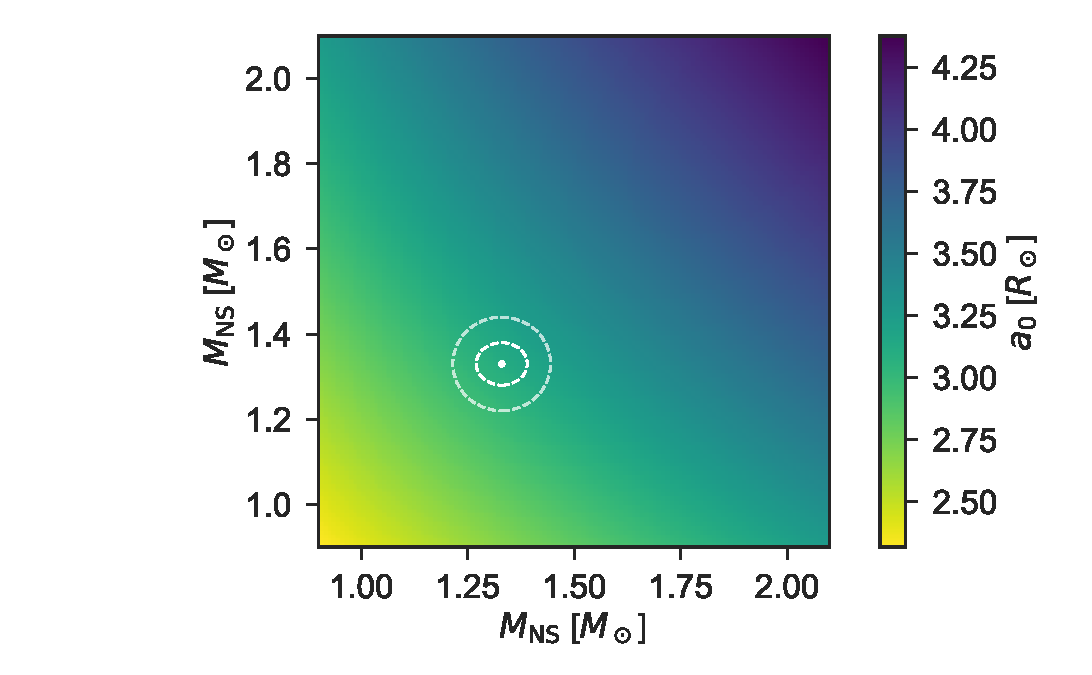
\includegraphics[width=9cm]{figures/prog_sep.pdf}
	\caption{Constraints on the initial progenitor separation, given binary constituent masses. As can be seen, a heavier system will inspiral faster, leading to a weaker constraint on the initial separation of the binary. The most probable value, the 68 per cent, and 98 percent posterior predictive intervals of the NS binary mass distribution from \citet{Kiziltan2013} are shown with the dashed ellipses, which corresponds to a constraint on maximal initial separation of $a_0 <3.1^{+0.2(+0.4)}_{-0.2(-0.4)}~R_\odot$, respectively.}
	\label{fig:prog_sep}
\end{figure}

Using the inferred stellar population age from our SED fit, we obtain a less
robust limit on the initial separation of $a_0 < 2.0^{+0.4}_{-0.4}~R_\odot$.
However, this does not account for the possibility there could be an underlying
stellar population of older stars from a previous star-formation episode. To
investigate the possible impact of the presence of an old stellar population, we
followed \citet{Papovich2001} and re-fitted the observed SED with the best-fit
template to which an additional stellar population of old stars was added. For
each template, this old population was set as the SSP with the same parameters as
the best-fit SED except the age, which was set to the age of the Universe at
the observed redshift. In principle, this can constrain the maximum contribution
of old populations within the photometric error bars \citep[see][for
details]{Papovich2001}. We find a negligible contribution to the stellar mass
(i.e. variations much smaller than the statistical uncertainty associated with
the best-fit template).

The delay time between formation and explosion is well accommodated by the
models of \citet{Belczynski2006}, although the longest delay times are excluded.
This is especially true given the late type nature of the host
\citep{OShaughnessy2008}. The same holds, if NS binaries are primarily formed
through dynamical interactions in globular clusters \citep{Lee2010, Church2011}.

%%%%%%%%%%%%%%%%%%%%%%%%%%%%%%%%%%%%%%%%%%%%%%%%%%%%%%%%%%%%%%%%%%%%%%%%%%%%
\section{Conclusions}
%%%%%%%%%%%%%%%%%%%%%%%%%%%%%%%%%%%%%%%%%%%%%%%%%%%%%%%%%%%%%%%%%%%%%%%%%%%%

We have here provided a revised, spectroscopic redshift measurement for the
short GRB~111117A based on host galaxy emission lines setting it at $z = 2.211
\pm 0.001$. This value supersedes the previous photometric redshift estimates of
\citet{Margutti2012} and \citet{Sakamoto2013}. The erroneous best-fit SED
redshift of previous authors is attributed to a discrepancy in the measured
$z$-band magnitude, and highlights the importance of deep spectroscopic studies
of sGRB hosts at medium resolution.

Using the new distance, the X-ray derived $N_\mathrm{H,X}$ towards GRB~111117A
is the highest within a complete sample of sGRBs and is consistent with the
$N_\mathrm{H,X}-z$ evolution traced by the sight lines of lGRBs. The SFR of the
host is in the upper end of the sGRB host SFR distribution and no significant
amount of dust is present. The high $N_\mathrm{H,X}$ is at odds with the large
projected host offset and the absence of dust. One possible explanation could be
that GRB~111117A is formed through a prompt channel of sGRB formation and
originates in an (unseen) star forming region located in the outskirts of the
host, or a localized region of high \hi~density along the line of sight.

Although a single burst carries little leverage in terms of constraining the
redshift distribution of sGRB, the high redshift of GRB~111117A needs to be
accommodated in progenitor models. A lognormal delay time model predicts a very
low volumetric density of bursts at $z \sim 2$, whereas a power law delay time
model peaks near the GRB~111117A redshift. If more sGRBs are at similarly high
redshifts, but are missed due to the faintness of their hosts and afterglows, a
lognormal delay time model will be disfavored. Compared to a complete sample of
\textit{Swift}-detected sGRB, the host of GRB~111117A is more luminous than 80
per cent of sGRB hosts with measured luminosities. Assuming a host brightness
redshift determination threshold, for between 43 and 71 per cent of the sample
hosts, we would be unable to determine a redshift should they be at a similar
redshift of GRB~111117A. This could indicate that, potentially, a significant
fraction of \textit{Swift}-detected sGRBs are at high $z$, but with redshifts
unknown due to host faintness.

Using the age of the universe at the time of explosion allows us to set
constraints on the maximal separation between the engine constituents at the
time of formation. We find that the maximal separation of two NSs at system
formation time is $a_0 < 3.1~R_\odot$, which excludes some of the formation
channels with the longest timescales.

All data, code and calculations related to the paper along with the
paper itself are available at \url{https://github.com/jselsing/GRB111117A}.

\begin{acknowledgements}
We thank the anonymous referee for a constructive report. 
%
We thank Jens Hjorth and Lise Christensen for useful discussions regarding the interpretation of this event. We thank Mathieu Puech for testing the possible contribution from an older stellar population in the SED. We thank Peter Laursen for fruitful discussions regarding the \lya~escape fraction.
%	
TK acknowledges support through the Sofja Kovalevskaja Award to P. Schady.
%
SDV is supported by the French National Research Agency (ANR) under contract ANR-16-CE31-0003 BEaPro.
%
PDA, SCo, acknowledge support from ASI grant I/004/11/3.
%
JJ acknowledges support from NOVA and NWO-FAPESP grant for advanced
instrumentation in astronomy.
%
NRT and KW acknowledge support from STFC Consolidated
Grant ST/N000757/1.
%
CT acknowledges support from a Spanish National Research Grant of Excellence
under project AYA 2014-58381-P and funding associated to a Ramón y Cajál
fellowship under grant number RyC-2012-09984.
%
AdUP acknowledges support from a Ramón y Cajal fellowship, a BBVA Foundation
Grant for Researchers and Cultural Creators, and the Spanish Ministry of Economy
and Competitiveness through project AYA2014-58381-P.
%
ZC acknowledges support from the Spanish research project AYA 2014-58381-P and
support from Juan de la Cierva Incorporaci\'on fellowships IJCI-2014-21669.
%
RSR acknowledges AdUP's BBVA Foundation Grant for Researchers and Cultural
Creators and support from ASI (Italian Space Agency) through the Contract n. 2015-046-R.0 and from European Union Horizon 2020 Programme under the AHEAD project (grant agreement n. 654215).
%
This research made use of Astropy, a community-developed core Python package for Astronomy \citep{TheAstropyCollaboration2013}. The analysis and plotting has been achieved using the Python-based packages Matplotlib \citep{Hunter2007}, Numpy, and Scipy \citep{VanderWalt2011}, along with other community-developed packages.
%
This work made use of observations obtained with the Italian 3.6 m Telescopio Nazionale Galileo (TNG) operated on the island of La Palma by the Fundaci\'on Galileo Galilei of the INAF (Istituto Nazionale di Astrofisica) at the Spanish Observatorio del Roque de los Muchachos of the Instituto de Astrof\'isica de Canarias.
%
Based on data from the GTC Archive at CAB (INTA-CSIC) and on observations obtained at the Gemini Observatory, which is operated by the Association of Universities for Research in Astronomy, Inc., under a cooperative agreement with the NSF on behalf of the Gemini partnership: the National Science Foundation (United States), the National Research Council (Canada), CONICYT (Chile), Ministerio de Ciencia, Tecnología e Innovación Productiva (Argentina), and Ministério da Ciência, Tecnologia e Inovação (Brazil).

\end{acknowledgements}

\bibliographystyle{mnras}
\bibliography{GRB111117A}

\end{document}


